% arara: xelatex
% arara: biber
% arara: xelatex
% arara: xelatex

%%%%%%%%%%%%%%%%%%%%%%%%%%%%%%%%%%%%%%%%%
% CLASS OPTIONS
% language: czech/english/slovak
% thesis type: bachelor/master/dissertation
% color: bw for black&white OR no option for default color scheme
% electronic (oneside) or printed (twoside), twoside is default
% paragraph - if passed, this optional argument sets paragraphs as the deepest level of headers, styles it, numbers it and adds it to Table of Content. Use with care! Normally, it is considered unwise to use it, since its too deep.
%%%%%%%%%%%%%%%%%%%%%%%%%%%%%%%%%%%%%%%%%
\documentclass[english,bachelor,unicode,twoside]{ctufit-thesis}

%%%%%%%%%%%%%%%%%%%%%%%%%%%%%%%%%%
% FILL IN THIS INFORMATION
%%%%%%%%%%%%%%%%%%%%%%%%%%%%%%%%%%
\ctufittitle{TinyC Compiler Frontend}
\ctufitauthorfull{Mykhailo Anisimov}
\ctufitauthorsurnames{Anisimov} 
\ctufitauthorgivennames{Mykhailo}
\ctufitsupervisor{Ing.\,Petr Máj,\,Ph.D.}
\ctufitdepartment{Department of Software Engineering}
\ctufityear{2025}
\ctufitdeclarationplace{Prague}
\ctufitdeclarationdate{\today}
\ctufitabstractCZE{Tato práce představuje překladový frontend pro programovací jazyk \texttt{tinyC} používaný v kurzu NI-GEN, navržený k usnadnění implementace backendu v různých programovacích jazycích. Frontend nabízí jak standardizované JSON rozhraní pro jazykově nezávislý vývoj backendu, tak i přímé použití C++ knihovny. Na základě analýzy technologií parserů a reprezentací AST implementace zahrnuje rekurzivní sestupný parser s LL(1) gramatikou, sledování pozic ve zdrojovém kódu a definované JSON schéma. Díky své přehledné architektuře a dokumentaci slouží tento frontend jako výukový nástroj při zachování rozšiřitelnosti pro budoucí vylepšení.}
\ctufitabstractENG{This thesis presents a compiler frontend for the \texttt{tinyC} programming language used in the NI-GEN course, designed to facilitate backend implementation in diverse programming languages. The frontend offers both a standardized JSON interface for language-agnostic backend development and a direct C++ library option. Based on analysis of parser technologies and AST representations, the implementation features a recursive descent parser with LL(1) grammar, source location tracking, and a defined JSON schema. With its clean architecture and documentation, this frontend serves as an educational tool while maintaining extensibility for future enhancements.}
\ctufitkeywordsCZE{překladový frontend, AST, LL1 parser, \texttt{tinyC}, OOP, serializace JSON, jazykově nezávislý návrh}
\ctufitkeywordsENG{compiler frontend, AST, recursive descent parser, \texttt{tinyC}, OOP, JSON serialization, language-agnostic design}
%%%%%%%%%%%%%%%%%%%%%%%%%%%%%%%%%%
% END FILL IN
%%%%%%%%%%%%%%%%%%%%%%%%%%%%%%%%%%

%%%%%%%%%%%%%%%%%%%%%%%%%%%%%%%%%%
% CUSTOMIZATION of this template
% Skip this part or alter it if you know what you are doing.
%%%%%%%%%%%%%%%%%%%%%%%%%%%%%%%%%%

\RequirePackage{iftex}[2020/03/06]
\iftutex % XeLaTeX and LuaLaTeX
    \RequirePackage{ellipsis}[2020/05/22] %ellipsis workaround for XeLaTeX
% \else
%     \errmessage{Only compilation with XeLaTeX or LuaLaTeX is allowed}
%     \stop
\fi

% hyperlinks
\hypersetup{
    pdfpagelayout=TwoPageRight,
    colorlinks=false,
    allcolors=decoration,
    pdfborder={0 0 0.1}
}

% uncomment the following to hide all hyperlinks
%\hypersetup{hidelinks}

% uncomment the following to change the color of all hyperlinks to CTU blue
%\hypersetup{allbordercolors=decoration}

\RequirePackage{pdfpages}[2020/01/28]

%%%%%%%%%%%%%%%%%%%%%%%%%%%%%%%%%%
% CUSTOMIZATION of this template END
%%%%%%%%%%%%%%%%%%%%%%%%%%%%%%%%%%


%%%%%%%%%%%%%%%%%%%%%%
% DEMO CONTENTS SETTINGS
% You may choose to modify this part.
%%%%%%%%%%%%%%%%%%%%%%
\usepackage{dirtree}
\usepackage{lipsum,tikz}
\usepackage[style=iso-numeric]{biblatex}
\addbibresource{text/bib-database.bib}
\usepackage{xurl}
\usepackage{listings} % typesetting of sources
\usepackage{syntax}
\usepackage{tabularx}
\usepackage{longtable} % for tables that span multiple pages
\usepackage{minted}
\usepackage{etoolbox} % Required for patching minted
\makeatletter
\patchcmd{\minted@pygmentize}
  {\FV@BreakAfterTokenfalse}
  {\FV@BreakAfterTokentrue}
  {}{}
\makeatother
\counterwithin{listing}{chapter} % testing for now
\usepackage{csquotes}
\usepackage{pgfplots}

\usetikzlibrary{arrows,shapes,positioning,fit,decorations.pathreplacing,backgrounds}
\usepackage{graphicx}
\graphicspath{{figures/}}
\pgfplotsset{compat=1.18}
\pdfminorversion=5


% Custom commands below
\usepackage{amsmath}
\allowdisplaybreaks    % Allows align/alignat to break across pages if needed


%%%%%%%%%%%%%%%%%%%%%%
% DEMO CONTENTS SETTINGS END
%%%%%%%%%%%%%%%%%%%%%%
\begin{document}
\frontmatter\frontmatterinit % do not remove these two commands

\thispagestyle{empty}\maketitle\thispagestyle{empty}\cleardoublepage % do not remove these four commands

\includepdf[pages={1-}]{Assignment.pdf} % replace this file with your thesis assignment generated from ProjectsFIT

\imprintpage % do not remove this command
\stopTOCentries
%%%%%%%%%%%%%%%%%%%%%%
% list of other contents END
%%%%%%%%%%%%%%%%%%%%%%

%%%%%%%%%%%%%%%%%%%
% ACKNOWLEDGMENT
% FILL IN / MODIFY
% This is a place to thank people for helping you. It is common to thank your supervisor.
%%%%%%%%%%%%%%%%%%%
\begin{acknowledgmentpage}
    I would like to sincerely thank my supervisor, Ing. Petr Máj, Ph.D., for his guidance and invaluable support throughout this thesis. My deepest gratitude also goes to my parents, whose continuous support and encouragement have provided me with the opportunity to study abroad and pursue my academic and personal growth.
\end{acknowledgmentpage}
%%%%%%%%%%%%%%%%%%%
% ACKNOWLEDGMENT END
%%%%%%%%%%%%%%%%%%%


%%%%%%%%%%%%%%%%%%%
% DECLARATION
% FILL IN / MODIFY
%%%%%%%%%%%%%%%%%%%
% INSTRUCTIONS
% ENG: choose one of approved texts of the declaration. DO NOT CREATE YOUR OWN. Find the approved texts at https://courses.fit.cvut.cz/SFE/download/index.html#_documents (document Declaration for FT in English)
\begin{declarationpage}
I hereby declare that the presented thesis is my own work and that I have cited all sources of
information in accordance with the Guideline for adhering to ethical principles when elaborating an
academic final thesis.

I acknowledge that my thesis is subject to the rights and obligations stipulated by the Act No.
121/2000 Coll., the Copyright Act, as amended, in particular the fact that the Czech Technical
University in Prague has the right to conclude a license agreement on the utilization of this thesis as
a school work pursuant of Section 60 (1) of the Act.

I declare that I have used AI tools during the preparation and writing of my thesis. I have verified
the generated content. I confirm that I am aware that I am fully responsible for the content of the
thesis.
\end{declarationpage}
%%%%%%%%%%%%%%%%%%%
% DECLARATION END
%%%%%%%%%%%%%%%%%%%

\printabstractpage % do not remove this command


\tableofcontents % do not remove this command
%%%%%%%%%%%%%%%%%%%%%%
% list of other contents: figures, tables, code listings, algorithms, etc.
% add/remove commands accordingly
%%%%%%%%%%%%%%%%%%%%%%
\listoffigures % list of figures
\begingroup
\let\clearpage\relax
\listoftables % list of tables
\thectufitlistingscommand
\endgroup

%%%%%%%%%%%%%%%%%%%
% ABBREVIATIONS
% FILL IN / MODIFY
% OR REMOVE ENTIRELY
% List the abbreviations in lexicography order.
%%%%%%%%%%%%%%%%%%%
\chapter{\thectufitabbreviationlabel}

\begin{tabular}{rl}
    ADT   & Algebraic Data Type \\
    AST   & Abstract Syntax Tree \\
    BNF   & Backus-Naur Form \\
    CBOR  & Concise Binary Object Representation \\
    CFG   & Context-Free Grammar \\
    CFL   & Context-Free Language \\
    DFA   & Deterministic Finite Automaton \\
    DTD   & Document Type Definition \\
    IDE   & Integrated Development Environment \\
    IR    & Intermediate Representation \\
    JSON  & JavaScript Object Notation \\
    LL(1) & Left-to-right, Leftmost derivation, 1 token lookahead \\
    LALR  & Look-Ahead LR parser \\
    LR    & Left-to-right, Rightmost derivation \\
    LSP   & Language Server Protocol \\
    NFA   & Non-deterministic Finite Automaton \\
    OOP   & Object-Oriented Programming \\
    PEG   & Parsing Expression Grammar \\
    SLR   & Simple LR parser \\
    XML   & eXtensible Markup Language \\
    XSLT  & XML Stylesheet Language Transformations \\
\end{tabular}
%%%%%%%%%%%%%%%%%%%
% ABBREVIATIONS END
%%%%%%%%%%%%%%%%%%%
\resumeTOCentries
\mainmatter\mainmatterinit % do not remove these two commands
%%%%%%%%%%%%%%%%%%%
% THE THESIS
% MODIFY ANYTHING BELOW THIS LINE
%%%%%%%%%%%%%%%%%%%




% Introduction
\chapter{Introduction}

The primary aim of this thesis is to provide a compiler frontend for the \texttt{tinyC} language that simplifies backend implementation for students in the NI-GEN course. By delivering a standardized frontend capable of generating a language-agnostic abstract syntax tree (AST) in a JSON format, students can focus exclusively on backend implementation, optimization techniques, and code generation in their preferred programming language.


\section{Background and Motivation}

The NI-GEN: Code Generators course at the Czech Technical University is designed to teach both theoretical and practical aspects of compiler backend development. According to the course materials, students are expected to ``become acquainted with both theoretical and practical aspects of backend of an optimizing programming language compiler.'' Emphasizing hands-on experience, the course notes that ``the beauty of compilers comes in part from the fact that here, the saying that 'the devil lies in the details' is more pronounced than in many other parts of CS.''

To fulfill course requirements, students implement a compiler for a small language called \texttt{tinyC}, covering aspects such as:
\begin{itemize}
\item Syntax and semantic descriptions
\item Parser
\item Type checker
\item Translation to LLVM IR
\item Optimizations
\item Code generation for the idealized t86 target
\end{itemize}

While this approach places considerable demands on students to develop both frontend and backend components within a single term. Given that the course predominantly emphasizes backend development, providing a standardized, high-quality frontend would greatly benefit students, allowing them to concentrate on backend-specific tasks such as optimization and code generation.

\section{Problem Statement}

The current structure of the NI-GEN course assignments, which requires students to implement both frontend and backend components, poses several challenges:

\begin{enumerate}
    \item Students are provided with an existing parser written in C++, which is of poor quality and contains implementation errors. Consequently, students are forced not only to debug and improve this parser but also to implement the middle and backend in C++, a language in which many may lack sufficient proficiency.
    \item Limited time within a single-term course restricts in-depth exploration of backend optimization techniques.
    \item Implementing a parser and AST diverts focus from backend-centric learning objectives related to optimization and code generation.
\end{enumerate}

Thus, there is a clear necessity for a standardized frontend implementation for the \texttt{tinyC} language, facilitating backend development independently of the programming language used.

\section{Project Goals}

This thesis addresses these challenges by developing a compiler frontend for the \texttt{tinyC} language. The key objectives are:

\begin{itemize}
\item Developing a lexer and parser that conform precisely to the defined \texttt{tinyC} grammar.
\item Designing a well-structured and extensible AST.
\item Providing a library interface suitable for direct integration primarily into C++ projects, along with a standalone executable outputting the AST in a standardized, language-agnostic JSON format.
\item Including detailed source location information for improved debugging and error reporting.
\item Ensuring testing, clear documentation, and maintainable implementation.
\end{itemize}

With these objectives, the project aims to streamline frontend tasks, enabling students to allocate more resources towards mastering backend compiler techniques.

\section{Expected Contributions}

The thesis will provide several significant contributions:

\begin{itemize}
\item An extensive analysis of existing parser technologies and language-agnostic AST formats.
\item A robust, object-oriented AST design promoting easy traversal and modification.
\item A standardized and language-agnostic JSON representation of the AST, enabling flexibility in backend implementation.
\item A thoroughly tested lexer and parser implementation for \texttt{tinyC} in C++.
\item Comprehensive documentation and examples to facilitate integration into students' projects.
\end{itemize}

\section{Thesis Structure}

The remaining chapters of this thesis are structured as follows:

\begin{itemize}
    \item \textbf{Chapter 2:} \textit{Theoretical Background} introduces fundamental compiler theory, particularly lexical analysis, parsing methods, and AST structures relevant to \texttt{tinyC}.
    
    \item \textbf{Chapter 3:} \textit{Analysis of Existing Solutions} reviews current parser technologies and AST representations, and evaluates how well they meet the needs of this project.
    
    \item \textbf{Chapter 4:} \textit{Design Requirements \& Architecture} details the architecture of the \texttt{tinyC} compiler frontend, including AST class definitions, the visitor pattern, and the JSON format.
    
    \item \textbf{Chapter 5:} \textit{Evaluation} compares the developed frontend with existing solutions, evaluating its effectiveness, usability, and overall improvements.
    
    \item \textbf{Chapter 6:} \textit{Conclusion} summarizes the project's achievements and outlines possible future enhancements and extensions.
\end{itemize}




% Theoretical Background
\chapter{Theoretical Background}

The construction of robust and efficient compilers relies heavily on a strong theoretical foundation. This chapter aims to establish the importance of these theoretical underpinnings by exploring the key areas that are fundamental to understanding and building the frontend of a compiler. 
These areas include the principles of formal languages, the distinct phases of the compilation process, the intricacies of lexical analysis, the methodologies of syntax analysis, and the design considerations for abstract syntax trees. 

A solid grasp of these theoretical concepts empowers compiler developers to make informed design decisions, effectively troubleshoot challenges, and ultimately create reliable and performant language processing tools. The ability to build a compiler from its foundational principles, as well as to leverage existing compiler construction tools and understand their inherent limitations, is significantly enhanced by a comprehensive theoretical understanding.

\section{Formal Languages}

\begin{definition}
\textbf{Formal language} is a precisely defined set of strings composed from a finite alphabet, with their structure and validity governed by a specific set of rules known as a formal grammar\cite{aho2007compilers}.
\end{definition}

Unlike natural languages, which evolve organically and often contain ambiguities, formal languages are intentionally designed for specific applications, such as mathematics, chemistry, and, most importantly for our context, programming. The notation employed by mathematicians to express relationships between numbers and symbols, for instance, constitutes a formal language adept at its intended purpose. Similarly, programming languages are formal languages meticulously crafted to express computations in an unambiguous manner \cite{runestone-formal-natural-languages}.

The fundamental building blocks of a formal language include a finite set of symbols known as the alphabet, from which finite sequences (strings or words) are constructed, and a subset of these strings that constitutes the language itself. The syntax of a formal language determines which strings are well‑formed according to a predefined set of production rules \cite{aho2007compilers, runestone-formal-natural-languages}. The design of a programming language necessitates a precise syntax to guarantee each program has a unique interpretation by the compiler.

\subsection{Types of Formal Languages}

Formal languages can be categorised into different types based on the complexity of their defining grammars, often visualised through the Chomsky hierarchy illustrated in Figure~\ref{figure:chomsky}. Within this hierarchy, regular languages and context‑free languages hold particular significance for compiler frontends \cite{aho2007compilers}.

\begin{figure}[ht]
\centering
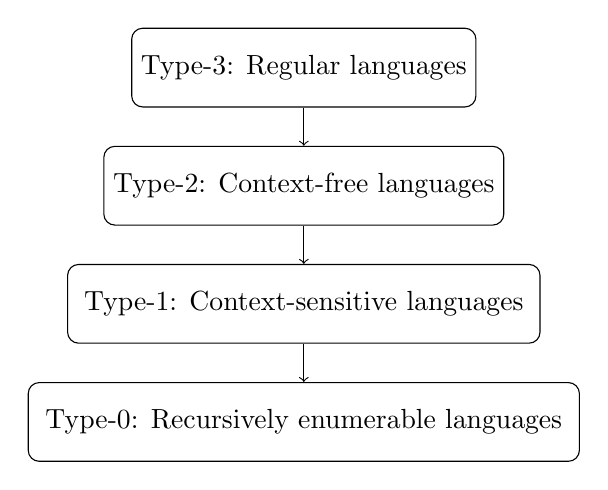
\begin{tikzpicture}[node distance=1.5cm]
\node (type3) [draw, rectangle, rounded corners=4pt, minimum width=4cm, minimum height=1cm] {Type‑3: Regular languages};
\node (type2) [draw, rectangle, rounded corners=4pt, minimum width=5cm, minimum height=1cm, below of=type3] {Type‑2: Context‑free languages};
\node (type1) [draw, rectangle, rounded corners=4pt, minimum width=6cm, minimum height=1cm, below of=type2] {Type‑1: Context‑sensitive languages};
\node (type0) [draw, rectangle, rounded corners=4pt, minimum width=7cm, minimum height=1cm, below of=type1] {Type‑0: Recursively enumerable languages};
\draw[->] (type3) -- (type2);
\draw[->] (type2) -- (type1);
\draw[->] (type1) -- (type0);
\end{tikzpicture}
\caption{Chomsky hierarchy of formal languages}
\label{figure:chomsky}
\end{figure}

\subsubsection*{Regular Languages}
Regular languages are the simplest in the hierarchy and can be defined using regular expressions, which offer a concise way to describe patterns of strings recognised by finite automata. In compilers, they are primarily used in lexical analysis to define tokens such as keywords, identifiers and operators \cite{aho2007compilers}.

\subsubsection*{Context‑Free Languages (CFLs)}
Context‑free languages, defined by context‑free grammars comprising production rules, are recognised by pushdown automata. The syntactic structure of programming languages—including hierarchical statements, expressions and control constructs—is typically defined using CFGs, and parsing relies on these principles \cite{kent-context-free-grammars-pda, aho2007compilers}.

While context‑sensitive and recursively enumerable languages appear in the Chomsky hierarchy, their direct relevance to compiler frontends is limited. Regular languages suffice for token recognition, whereas the intricate syntactic structures of programming languages demand the expressive power of context‑free languages.

\subsection{Key Properties of Formal Languages}

Understanding syntax, semantics and ambiguity is essential for comprehending how compilers process source code. Syntax governs token formation and program structure, semantics addresses the meaning and consistency checks during semantic analysis, and ambiguity—where a grammar permits multiple parse trees for the same string—is minimised in language design to ensure predictable compiler behaviour \cite{aho2007compilers}.

\subsection{The Significance of Formal Language Theory}

Formal language theory provides the mathematical tools and methodologies for specifying and implementing lexical analysers (via regular expressions and finite automata) and parsers (via context‑free grammars and parsing techniques). It guides the selection of appropriate formalisms, ensuring that compiler design proceeds systematically and reliably.

\pagebreak


\section{The Compilation Process}

The process of compiling a program is typically structured as a sequence of distinct phases, each responsible for a specific transformation of the source code as it progresses towards becoming executable machine code. These phases generally include Lexical Analysis (Scanning), Syntax Analysis (Parsing), Semantic Analysis, Intermediate Code Generation, Code Optimisation, and Code Generation (see Table~\ref{tab:compilation-phases}).


\begin{enumerate}
    \item \textbf{Lexical Analysis (Scanning):} This initial phase reads the source code character by character and groups these characters into meaningful units called lexemes. For each lexeme, the lexical analyser produces a token, which represents a category of lexical units such as keywords, identifiers, operators, and literals \cite{aho2007compilers}. It also typically removes whitespace and comments from the source code \cite{aho2007compilers}.
    \item \textbf{Syntax Analysis (Parsing):} The parser takes the stream of tokens produced by the lexical analyser and checks if this sequence of tokens adheres to the grammatical rules of the programming language. If the syntax is correct, the parser constructs a parse tree or an Abstract Syntax Tree (AST) that represents the hierarchical structure of the program \cite{aho2007compilers}.
    \item \textbf{Semantic Analysis:} This phase checks the program for semantic correctness, ensuring that the program makes sense according to the language's rules. This can involve type checking, verifying that variables are declared before use, and ensuring that operations are applied to compatible data types \cite{aho2007compilers}.
    \item \textbf{Intermediate Code Generation:} After semantic analysis, the compiler may generate an intermediate representation of the program. This representation is often a low-level, machine-independent code that facilitates optimisation and code generation for various target architectures \cite{aho2007compilers}.
    \item \textbf{Code Optimisation:} This optional phase aims to improve the intermediate code to make the program run faster or use fewer resources. Various optimisation techniques can be applied at this stage \cite{aho2007compilers}.
    \item \textbf{Code Generation:} The final phase translates the optimised intermediate code into the target machine code or assembly language that can be executed by the computer \cite{aho2007compilers}. This phase also involves tasks like register allocation and instruction scheduling.
\end{enumerate}


\begin{table}[t]
  \centering
  \begin{tabularx}{\textwidth}{|
      >{\raggedright\arraybackslash}X|
      >{\raggedright\arraybackslash}X|
      >{\raggedright\arraybackslash}X|
      >{\raggedright\arraybackslash}X|
    }
    \hline
    \textbf{Phase Name} & \textbf{Input} & \textbf{Output} & \textbf{Key Tasks} \\
    \hline\hline
    Lexical Analysis (Scanning) &
    Source code &
    Stream of tokens &
    Reads source code, groups characters into lexemes, produces tokens, removes whitespace/comments, reports errors. \\
    \hline
    Syntax Analysis (Parsing) &
    Stream of tokens &
    Parse tree or AST &
    Verifies token sequence against grammar, constructs parse tree/AST, reports syntax errors. \\
    \hline
    Semantic Analysis &
    Parse tree or AST &
    Annotated AST &
    Checks type and scope rules, annotates AST with semantic information. \\
    \hline
    Intermediate Code Generation &
    Annotated AST &
    Intermediate representation (IR) &
    Emits machine-independent IR for optimisation and code generation. \\
    \hline
    Code Optimisation &
    IR &
    Optimised IR &
    Applies transformations to improve performance or resource usage. \\
    \hline
    Code Generation &
    Optimised IR &
    Target machine code &
    Translates IR to assembly/machine code, performs register allocation and scheduling. \\
    \hline
  \end{tabularx}
  \caption{Phases of a Compiler and their key tasks}
  \label{tab:compilation-phases}
\end{table}

The compilation process is often divided into a frontend, which primarily deals with the analysis of the source code (lexical, syntax, and semantic analysis), and a backend, which focuses on the synthesis of the target code (intermediate code generation, optimisation, and code generation) \cite{aho2007compilers}. Throughout these phases, a symbol table is maintained to store information about identifiers (such as variable names, function names) used in the program, including their type, scope, and memory location \cite{aho2007compilers}. The modularity of the compilation process into these distinct phases allows for a structured approach to compiler design, where each phase can be developed and optimised with a degree of independence. Breaking down the complex task of translation into smaller, more manageable phases simplifies the overall development effort.

This thesis concentrates on the compiler frontend—namely lexical analysis and syntax analysis—as they form the theoretical basis for \texttt{tinyC}’s formal language processing. Lexical analysis tokenises the raw source into a sequence of symbols, while syntax analysis parses these tokens into a structured Abstract Syntax Tree (AST). Together, they ensure that source programs conform to the grammar of \texttt{tinyC}, providing the necessary structure for all subsequent compiler stages.


\pagebreak


\section{Lexical Analysis}

The lexical analyser, often referred to as a scanner or tokenizer, is the first phase in the compilation process. Its primary role is to read the source code, which is essentially a stream of characters, and to group these characters into meaningful sequences known as lexemes \cite{aho2007compilers}. 

\subsection{Responsibilities}

The lexical analyser is responsible for the following tasks:
\begin{enumerate}
  \item Produce a token for each identified lexeme, categorising it as a keyword (e.g.\ \texttt{if}, \texttt{while}), identifier (e.g.\ variable names), operator (e.g.\ \texttt{=}, \texttt{+}), literal (e.g.\ numbers, strings), or punctuation (e.g.\ parentheses, semicolons) \cite{aho2007compilers}.
  \item Remove whitespace (spaces, tabs, newlines) and comments, as they serve only to separate tokens and are not needed by the parser \cite{aho2007compilers}.
  \item Detect and report lexical errors, such as invalid characters or character sequences that do not match any token pattern \cite{aho2007compilers}.
  \item Store preliminary information about tokens—particularly identifiers—in the symbol table for later compiler phases \cite{aho2007compilers}.
  \item Track the location (line and column numbers) of each token for precise error reporting and downstream stages.
  \item Simplify the parser’s input by transforming the raw source code into a structured stream of tokens, thereby abstracting away character-level details.
\end{enumerate}

\subsection{Tokens, Lexemes, and Patterns}

To effectively understand the process of lexical analysis, it is crucial to distinguish between the concepts of tokens, lexemes, and patterns \cite{aho2007compilers}. 

Tokens are abstract categories (e.g.\ \texttt{KEYWORD}, \texttt{IDENTIFIER}, \texttt{INTEGER}); lexemes are the actual character sequences (e.g.\ \texttt{if}, \texttt{count}, \texttt{123}); and patterns are the regular expressions that define which lexemes belong to which token class \cite{aho2007compilers}.

\begin{table}[ht]
\centering
\begin{tabular}{lll}
\hline
Token             & Example lexemes      & Pattern (regex)                       \\
\hline
\texttt{KEYWORD}    & if, while, return    & \texttt{if|while|return|...}          \\
\texttt{IDENTIFIER} & count, tmp          & \texttt{[A-Za-z][A-Za-z_0-9]*}       \\
\texttt{INTEGER}    & 0, 123               & \texttt{[0-9]+}                       \\
\hline
\end{tabular}
\caption{Common token classes in \texttt{tinyC}}
\label{tab:lex-tokens}
\end{table}

Patterns are expressed using operators for concatenation, alternation (\texttt{|}), and repetition (\texttt{*}, \texttt{+}, \texttt{?}). For instance, \texttt{[A-Za-z_][A-Za-z_0-9]*} defines identifiers, while \texttt{[0-9]+} defines integer literals. Tools such as Lex or Flex convert these specifications into effective scanners \cite{aho2007compilers}.



\subsection{Specifying Tokens with Regular Expressions}

Regular expressions allow concise specification of token patterns \cite{aho2007compilers}. Key points include:
\begin{itemize}
  \item Identifiers: \texttt{[A-Za-z\_][A-Za-z\_0-9]*} matches names starting with a letter or underscore.
  \item Integer literals: \texttt{[0-9]+} matches one or more digits.
  \item Keywords: fixed strings such as \texttt{if}, \texttt{while}, \texttt{return}.
  \item Operators and punctuation: single- or multi-character sequences (e.g.\ \texttt{=}, \texttt{++}, \texttt{;}).
  \item Construction operators: concatenation, alternation (\texttt{|}), repetition (\texttt{*}, \texttt{+}, \texttt{?}).
\end{itemize}

% \subsection{Implementing Lexical Analysers using Finite Automata}

% The equivalence of regex and finite automata underpins scanner implementation \cite{aho2007compilers}. Main steps:
% \begin{itemize}
%   \item Convert each regular expression into an NFA.
%   \item Apply the powerset construction to transform NFAs into DFAs.
%   \item Build a transition table indexed by state and input symbol.
%   \item Scan input by following DFA transitions; reaching an accepting state emits the corresponding token.
%   \item Use the DFA’s accepting-state information to determine token type.
%   \item Report errors when no valid transition exists for an input character.
% \end{itemize}



% \subsection{Specifying Tokens with Regular Expressions}

% Regular expressions provide a powerful and concise means of specifying the patterns that define the various token types in a programming language \cite{aho2007compilers}. They are essentially a formal language used to describe sets of strings based on a defined set of rules \cite{aho2007compilers}. For example, a regular expression for an identifier might be \texttt{[a-zA-Z\_][a-zA-Z\_0-9]*}, which specifies a sequence of one or more letters, underscores, or digits, with the initial character being a letter or an underscore. Similarly, the regular expression for an integer literal could be \texttt{[0-9]+}, indicating one or more digits. Keywords, being fixed sequences of characters, have very simple regular expressions, such as \texttt{if} for the keyword "if" \cite{aho2007compilers}. Regular expressions utilise a set of operators to construct these patterns, including concatenation (joining sequences), alternation (specifying alternatives using the \texttt{|} operator), and repetition (using operators like \texttt{*} for zero or more occurrences, \texttt{+} for one or more, and \texttt{?} for zero or one) \cite{aho2007compilers}. The formal nature of regular expressions allows for their direct translation into finite automata, which are the underlying mechanism used for efficient scanning. Tools like Lex (and its more modern counterpart, Flex) are widely used in compiler construction to automate the process of generating a lexical analyser (a scanner) from a specification that primarily consists of a set of regular expressions, each associated with a specific token type \cite{aho2007compilers}. These tools take the regular expression specifications as input and automatically generate the code for a lexical analyser that can then scan the source code and produce the corresponding stream of tokens. This automation significantly simplifies the development of the lexical analysis phase of a compiler.

\subsection{Implementing Lexical Analysers using Finite Automata}

The theoretical equivalence between regular expressions and finite automata is fundamental to the implementation of lexical analysers \cite{aho2007compilers}. Regular expressions, as discussed, are used to specify the patterns for tokens. These regular expressions can be systematically converted into Non-deterministic Finite Automata (NFAs) \cite{aho2007compilers}.

An NFA is a finite automaton where for each state and each input symbol, there can be zero, one, or more next states. NFAs can also have transitions labelled with $\epsilon$ (epsilon), which represent transitions that can occur without consuming any input symbol \cite{aho2007compilers}. While NFAs are useful for specifying the lexical rules derived from regular expressions, they are often not the most efficient model for direct implementation. For implementation purposes, NFAs are typically converted into Deterministic Finite Automata (DFAs) using techniques such as the powerset construction \cite{aho2007compilers}. 

A DFA is a finite automaton that has exactly one transition for each input symbol from each state, and it does not have any $\epsilon$-transitions. This deterministic nature makes DFAs more straightforward and efficient to implement in a scanner.


A finite automaton (whether an NFA or a DFA) consists of a finite set of states, a set of input symbols (the alphabet), a transition function that defines how the automaton moves from one state to another based on the input symbol, a start state, and a set of accepting states \cite{aho2007compilers}. 
In the context of lexical analysis, the scanner operates by reading the input stream of characters, one at a time. Starting from the initial state of the DFA, the automaton transitions between states based on the input character. If, after reading a sequence of characters, the DFA ends up in an accepting state, it indicates that a token has been recognised. The type of the token is determined by the specific accepting state that was reached. 

The implementation of a DFA often involves the use of a transition table, which is a two-dimensional array where one dimension represents the current state and the other represents the input symbol. The entry in the table at the intersection of a state and an input symbol specifies the next state to which the automaton should transition \cite{aho2007compilers}. This table-driven approach provides an efficient mechanism for performing lexical analysis. The systematic conversion from regular expressions to NFAs and then to DFAs allows for an automated way to build the lexical analysis phase of a compiler, where token recognition is driven by well-defined state transitions based on the characters in the source code.

\pagebreak


\section{Syntax Analysis}

Syntax analysis, commonly known as parsing, is the second phase of the compilation process. It operates on the token stream produced by the lexical analyser and fulfils the following objectives \cite{aho2007compilers}:

\begin{enumerate}
\item \textbf{Syntax Verification:} Ensure the token sequence conforms to the language grammar.
\item \textbf{Structural Construction:} Build a hierarchical representation (parse tree or Abstract Syntax Tree).
\item \textbf{Error Reporting:} Detect and report syntactic errors in the source code.
\end{enumerate}

The parser examines the relationships and order of tokens to confirm that the source code adheres to the defined syntax. A successful parse yields a structured representation, which is essential for subsequent phases such as semantic analysis and intermediate code generation.

\subsection{Context-Free Grammars}

Context-free grammars (CFGs) formally specify the syntax of programming languages \cite{aho2007compilers}. A CFG consists of:

\begin{itemize}
\item \textbf{Terminal Symbols:} Basic tokens provided by the lexical analyser.
\item \textbf{Non-terminal Symbols:} Higher-level constructs (e.g. expressions, statements).
\item \textbf{Production Rules:} Definitions of how non-terminals expand into terminals and/or other non-terminals.
\item \textbf{Start Symbol:} The root non-terminal representing a complete program.
\end{itemize}

Derivation begins at the start symbol and proceeds by applying production rules until the input token sequence is generated. Table~\ref{tab:parse-tree-general} illustrates parse tree with its corresponding grammar.

\subsection{Top-Down and Bottom-Up Parsing}

Parsing techniques can be broadly classified into two categories: top-down and bottom-up approaches. As shown in Table~\ref{tab:td-vs-bu}, these methods differ significantly in their approach to constructing the parse tree.

\subsection{Top-Down Parsing Techniques}

Top-down parsing begins at the start symbol and works towards the input tokens, predicting productions to derive the input. Common methods include:

\subsubsection*{Recursive Descent Parsing}
Each non-terminal is implemented as a recursive function. Functions attempt to match tokens and call other functions for nested constructs. Backtracking may be required if a prediction fails \cite{aho2007compilers}.

\subsubsection*{LL(1) Parsing}
LL(1) parsers scan left-to-right, construct a leftmost derivation, and use one lookahead symbol. They rely on FIRST and FOLLOW sets and parsing tables to avoid backtracking \cite{aho2007compilers}.

\subsection{Bottom-Up Parsing Techniques}

Bottom-up parsing starts with tokens and reduces them to non-terminals, reconstructing a rightmost derivation in reverse. Key approach:

\subsubsection*{LR (Shift-Reduce) Parsing}
LR parsers use ACTION and GOTO tables to decide between \textit{shift} and \textit{reduce} operations. Variants include SLR, LALR, and LR(1) \cite{aho2007compilers}.

\begin{table}[ht!]
    \centering
    \renewcommand{\arraystretch}{1.2} 
    \begin{tabularx}{\textwidth}{%
        >{\raggedright\arraybackslash}X%
        >{\centering\arraybackslash}X%
      }
      \textbf{Explanation} 
        & \textbf{Parse Tree} \\
      \hline
      \vspace{0.5em}
      A CFG derivation can be visualised as a tree: the start symbol is at the root, and each application of a production rule adds children corresponding to the symbols on the right-hand side. For instance, given:
      \[
        S \;\rightarrow\; A\,B,\quad A\;\rightarrow\;a,\quad B\;\rightarrow\;b,
      \]
      the parse tree captures exactly that structure, showing how \(S\) expands into \(A\) and \(B\), and then into terminals \(a\) and \(b\). 
      \vspace{0.5em}
        & 
      \vspace{3em}
      \begin{tikzpicture}[level distance=1.2cm, sibling distance=1.2cm]
        \node {S}
          child { node {A}
            child { node {a} }
          }
          child { node {B}
            child { node {b} }
          };
      \end{tikzpicture}
      \vspace{1em} \\
    \end{tabularx}
    
    \caption{Parse tree for the grammar \(S \rightarrow AB,\;A\rightarrow a,\;B\rightarrow b\).}
    \label{tab:parse-tree-general}
\end{table}  

\begin{table}[ht!]
    \centering
    \renewcommand{\arraystretch}{1.2}
    \begin{tabularx}{\textwidth}{|
        >{\raggedright\arraybackslash}p{0.2\textwidth}|
        >{\raggedright\arraybackslash}X|
        >{\raggedright\arraybackslash}X|
      }
      \hline
      \textbf{Feature} & \textbf{Top-Down Parsing} & \textbf{Bottom-Up Parsing} \\
      \hline
      Starting Point
        & Start symbol (root of parse tree)
        & Input tokens (leaves of parse tree) \\
      \hline
      Derivation Type
        & Leftmost derivation
        & Rightmost derivation in reverse \\
      \hline
      Handling of Left Recursion
        & Requires elimination of left recursion
        & Can handle left-recursive grammars \\
      \hline
      Common Techniques
        & Recursive Descent, LL(1) Parsing, Predictive Parsing
        & LR Parsing (SLR, LALR, LR), Shift-Reduce Parsing, Operator Precedence Parsing \\
      \hline
      Prediction of Production
        & Predicts the next production to apply
        & Postpones the decision until the entire right side is seen \\
      \hline
      Control
        & Explicitly constructs the parse tree from the top
        & Attempts to reduce the input to the start symbol \\
      \hline
    \end{tabularx}
    \caption{Comparison of Top-Down and Bottom-Up Parsing}
    \label{tab:td-vs-bu}
\end{table}

\pagebreak

\section{Abstract Syntax Tree}

The Abstract Syntax Tree (AST) is a tree-like data structure representing the essential syntactic structure of a program's source code. It is constructed by the syntax analysis phase of a compiler, immediately after lexical analysis. The AST serves as a crucial intermediate representation for subsequent compiler phases: semantic analysis, intermediate code generation, and code optimisation. It abstracts away inessential concrete syntax details (e.g.\ parentheses, semicolons) to focus on core syntactic and semantic information \cite{aho2007compilers}.

\begin{figure}[hb!]
    \centering
    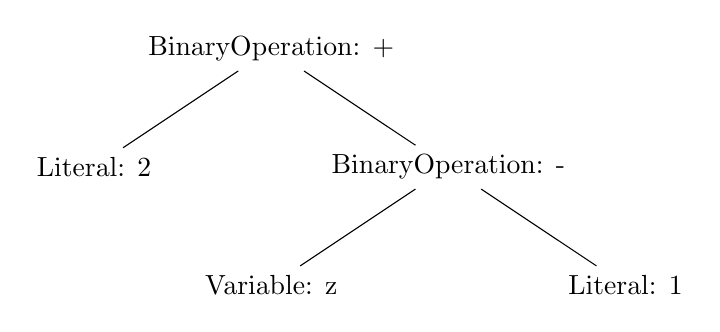
\begin{tikzpicture}[level distance=1.5cm, sibling distance=4.5cm]
      \node {BinaryOperation: +}
        child { node {Literal: 2} }
        child { node {BinaryOperation: -}
          child { node {Variable: z} }
          child { node {Literal: 1} }
        };
    \end{tikzpicture}
    \caption{AST of the expression \texttt{2 + (z - 1)}}
    \label{fig:ast-example}
\end{figure}

In an AST, each node represents a construct occurring in the source code \cite{aho2007compilers}. These constructs can include operators (e.g.\ addition, subtraction), variables, control flow statements (e.g.\ if-then-else, loops), function calls, and literals. The children of a node represent its components or operands. For instance, in an AST for the expression \texttt{2 + (z - 1)}, as shown in Figure~\ref{fig:ast-example}, the root node represents a binary addition operation, with two children: one for the literal value \texttt{2}, and one for a binary subtraction operation, which in turn has children representing the variable \texttt{z} and the literal value \texttt{1}. Each node stores information about its construct type and related data (e.g.\ variable names, literal values), encoding hierarchical relationships and operator precedence \cite{aho2007compilers}.

\subsection{Abstraction from Concrete Syntax}

The AST abstracts away inessential concrete syntax details present in a parse tree \cite{aho2007compilers}. It omits grouping parentheses, statement-terminating semicolons, and parsing-only non-terminals, retaining only the constructs needed for semantic understanding. By eliminating syntactic sugar and focusing on semantic content, the AST provides a cleaner, more manageable structure for semantic analysis and code generation \cite{aho2007compilers}.

\subsection{Further Compiler Stages}

As an intermediate representation, the AST bridges initial code analysis and later compiler phases. It underpins semantic analysis—checking types, scopes, and other constraints—by providing a traversable structure. The AST also forms the basis for generating machine-independent intermediate code and enables code optimisation techniques through its well-defined hierarchy. A carefully designed AST thus directly impacts the efficiency and correctness of generated target code \cite{aho2007compilers}.

\section{Conclusion}

This chapter has explored the fundamental theoretical concepts that underpin the frontend of a compiler. We have examined the principles of formal languages, which provide the mathematical framework for defining the syntax of programming languages. We have also discussed the compilation process as a sequence of phases, with a particular focus on lexical analysis, the process of breaking down the source code into tokens, and syntax analysis, which involves parsing these tokens according to the language's grammar. Finally, we delved into the design and importance of Abstract Syntax Trees, which serve as a crucial intermediate representation of the program's structure for subsequent compiler stages. These theoretical concepts are interconnected and collectively form the essential foundation for the design and implementation of efficient and reliable compiler frontends. The principles discussed here will be directly applicable and further elaborated upon in the subsequent chapters, where we will explore their application in the specific context of the \texttt{tinyC} compiler frontend.


% Analysis of Existing Solutions
\chapter{Analysis of Existing Solutions}

The development of a compiler frontend for educational purposes requires careful consideration of existing technologies, approaches, and best practices. This chapter examines various parser technologies, AST representations, serialization formats, and educational compiler frontends, with the aim of informing the design decisions for the \texttt{tinyC} frontend implementation.

\section{Parser Technologies}

Numerous approaches to parsing have been developed over the decades, each with its own advantages and trade-offs. This section analyzes the most relevant parser technologies from the perspective of educational compiler development.

\subsection{Handwritten Recursive Descent Parsers}

Recursive descent parsers represent one of the most straightforward approaches to parsing, implementing the grammar rules directly as a set of mutually recursive functions \cite{aho2007compilers}. Each function corresponds to a non-terminal in the grammar and is responsible for recognizing the corresponding syntactic construct.

For educational purposes, handwritten recursive descent parsers offer significant pedagogical value. Their directness creates a clear correspondence between grammar and code, making it easier for students to grasp the relationship between formal grammar specifications and implementation \cite{parr2010language}. They provide developers with fine-grained control over error messages, enabling more student-friendly diagnostic information \cite{holub1990compiler}. Additionally, their flexibility allows modifications to the grammar to be directly translated to code changes without requiring intermediary tools \cite{grune2012modern}.

Despite these advantages, handwritten parsers present certain challenges. They tend to be labor-intensive, requiring considerable manual coding, particularly for complex languages \cite{grune2012modern}. A significant technical limitation is their inability to handle left recursion directly, which necessitates grammar transformations \cite{aho2007compilers}. From a maintenance perspective, changes to the grammar often require coordinated modifications across numerous functions, increasing the risk of inconsistencies \cite{crenshaw1988lets}.

\subsection{Parser Generators}

Parser generators automate the creation of parsers from grammar specifications. Tools like ANTLR \cite{parr2013definitive}, Bison, and Yacc have long been used in compiler construction courses.

These tools offer significant advantages for compiler development. They enhance productivity by generating parser code directly from grammar specifications, substantially reducing implementation time \cite{levine2009flex}. Parser generators stand on a solid formal basis, implementing well-studied parsing algorithms with proven mathematical properties and performance characteristics \cite{aho2007compilers}. Additionally, many parser generators include grammar validation capabilities that check for potential issues such as ambiguities or conflicts, providing early feedback to developers before implementation begins \cite{parr2013definitive}.

Despite these benefits, parser generators present certain challenges in educational contexts. Students face a steeper learning curve as they must master both the grammar specification language and the integration patterns with the host language, adding cognitive load to the learning process \cite{sestoft2017programming}. An abstraction gap often emerges where the generated code obscures the connection between grammar and parsing logic, potentially hindering students' understanding of the underlying principles \cite{grune2012modern}. Furthermore, the default error messages produced by many parser generators tend to be cryptic and implementation-oriented rather than user-friendly, requiring significant additional work to make them accessible and helpful to students \cite{tratt2010parsing}.

\subsection{Parser Combinators}

Parser combinators represent a functional approach to parsing, where basic parsers are combined using higher-order functions to create more complex parsers \cite{hutton1992higher}. Libraries like Parsec for Haskell and parser-combinators for Scala exemplify this approach.

The composability of parser combinators constitutes one of their primary strengths, allowing simple parsers to be combined in modular ways to handle increasingly complex structures \cite{leijen2001parsec}. In statically typed languages, parser combinators benefit from type safety, ensuring that type errors in parser construction are identified at compile time rather than manifesting as runtime errors \cite{marlow2011haskell}. This approach also tends to produce readable code where the parsing logic closely resembles the grammar itself, enhancing maintainability and facilitating understanding of the relationship between grammar and implementation \cite{moors2008parser}.

Despite these merits, parser combinators come with certain drawbacks. Performance issues may arise in naive implementations due to excessive backtracking, potentially leading to exponential time complexity in worst-case scenarios \cite{leijen2001parsec}. Educational applications face a particular challenge in that parser combinators typically require familiarity with functional programming concepts, creating a potential barrier for students without this background \cite{sestoft2017programming}. Furthermore, advanced error recovery techniques—critical for providing helpful feedback to users—can be particularly difficult to implement in combinator-based parsers, often requiring specialized extensions to the basic combinator framework \cite{tratt2010parsing}.

\subsection{PEG Parsers}

Parsing Expression Grammars (PEGs) provide an alternative formalism to Context-Free Grammars, with ordered choice replacing the ambiguous choice of CFGs \cite{ford2004parsing}. PEG parsers often use packrat parsing techniques to achieve linear time complexity.

PEG parsers offer several distinctive advantages in parser implementation. Their ordered choice operator fundamentally eliminates parsing ambiguities by definition, as the first successful match is always chosen, creating deterministic behavior even with complex grammar constructs \cite{ford2004parsing}. Many PEG implementations combine lexical and syntactic analysis into a unified process, removing the traditional separation between scanner and parser phases and potentially simplifying the overall implementation \cite{grimm2006better}. Beyond the capabilities of traditional context-free grammar tools, PEGs possess expressive power that enables them to recognize some non-context-free languages, broadening the range of syntactic structures they can parse \cite{medeiros2014peg}.

These advantages, however, are counterbalanced by notable challenges. The ordered choice operator, while eliminating ambiguity, can lead to subtle and sometimes unexpected parsing behavior when grammar rules interact in complex ways \cite{tratt2010parsing}. Although packrat parsing achieves efficient linear time complexity, this comes at the cost of potentially high memory requirements due to the memoization of intermediate results \cite{ford2002packrat}. From a theoretical perspective, PEGs have a less established mathematical foundation compared to LR or LL parsing techniques, which have decades of theoretical analysis and optimization research behind them \cite{medeiros2014peg}.

\subsection{Comparative Analysis}

Table \ref{tab:parser-comparison} presents a comparison of these parser technologies across dimensions particularly relevant to educational compiler development.

\begin{table}[h]
    \centering
    \renewcommand{\arraystretch}{1.2}
    \caption{Comparison of Parser Technologies for Educational Use}
    \label{tab:parser-comparison}
    \begin{tabularx}{\textwidth}{|
        >{\raggedright\arraybackslash}p{2.6cm}|
        >{\centering\arraybackslash}X|
        >{\centering\arraybackslash}X|
        >{\centering\arraybackslash}X|
        >{\centering\arraybackslash}X|
      }
      \hline
      \textbf{Criterion} & \textbf{Recursive Descent} & \textbf{Parser Generators} & \textbf{Parser Combinators} & \textbf{PEG Parsers} \\
      \hline
      Implementation effort     & High                     & Low                       & Medium                        & Low                    \\
      \hline
      Error reporting quality   & Excellent                & Poor to Medium            & Medium                        & Medium                 \\
      \hline
      Educational clarity       & High                     & Medium                    & High (if functional programming is known) & Medium  \\
      \hline
      Grammar flexibility       & Medium                   & Medium to High            & High                          & High                   \\
      \hline
      Performance               & Good                     & Excellent                 & Variable                      & Good to Excellent      \\
      \hline
      Tool dependencies         & None                     & Required                  & Library only                  & Library or Generator   \\
      \hline
    \end{tabularx}
\end{table}  
  

For the \texttt{tinyC} frontend, considering its educational purpose and the need for high-quality error reporting, a recursive descent parser with predictive parsing techniques offers an appealing balance of clarity, control, and performance.

\pagebreak







\section{AST Representations}

The Abstract Syntax Tree (AST) serves as the central data structure in a compiler, bridging the parsing and semantic analysis phases. Various approaches to AST design and implementation exist, each with implications for educational compiler development.

\subsection{Object-Oriented Hierarchies}

Traditional object-oriented AST designs use class hierarchies, with a base node class and derived classes for specific language constructs \cite{gamma1995design}. This approach is common in compilers implemented in languages like C++, Java, and C\#.

Object-oriented AST hierarchies provide intuitive modeling where the class structure naturally maps to the syntactic categories of the language, creating clear parallels between the grammar and implementation \cite{appel2004modern}. Their extensibility allows new node types to be added by extending the hierarchy without disturbing existing code, facilitating incremental development \cite{gamma1995design}. Furthermore, their strong typing ensures operations are applied to appropriate nodes, catching many errors at compile time rather than runtime \cite{odersky2004overview}.

Despite these strengths, object-oriented hierarchies exhibit certain limitations. Their inherent rigidity means that adding new operations across the entire AST typically requires modifying every node class, violating the open-closed principle \cite{gamma1995design}. Implementation often demands substantial repetitive code for node constructors, accessors, and other boilerplate, increasing maintenance burden \cite{appel2004modern}. Additionally, correctly implementing the visitor pattern to address the operation extension problem requires careful attention to detail and introduces its own complexity \cite{gamma1995design}.


\subsection{Algebraic Data Types}

Languages that support algebraic data types (ADTs) offer an alternative approach to AST representation \cite{krishnamurthi2007programming}. This approach is common in functional languages like ML, Haskell, and increasingly in modern multi-paradigm languages.

ADTs enable notably concise AST definitions, often allowing the entire tree structure to be described in a fraction of the code required by object-oriented approaches \cite{krishnamurthi2007programming}. Their support for exhaustive pattern matching facilitates AST processing, with compilers typically warning about unhandled cases, reducing the risk of overlooking edge cases \cite{odersky2004overview}. The immutable nature of typical ADT implementations simplifies reasoning about AST transformations, eliminating concerns about unexpected state changes during processing \cite{okasaki1999purely}.

The ADT approach, however, faces significant practical challenges. Many mainstream languages used in education lack native ADT support, limiting the applicability of this approach in diverse educational settings \cite{krishnamurthi2007programming}. ADTs also suffer from the expression problem in reverse: while adding operations is straightforward, adding new node types requires modifying all functions that process the AST \cite{wadler1998expression}. From a performance perspective, naive ADT implementations may incur higher memory overhead compared to optimized object-oriented designs due to boxing and indirection \cite{appel2004modern}.


\subsection{Visitor Pattern Applications}

The Visitor pattern provides a way to separate algorithms from the objects they operate on, addressing some limitations of rigid class hierarchies \cite{gamma1995design}. It is commonly used for AST traversal and transformation.

The classic Visitor pattern defines a visitor interface with visit methods for each node type, enabling new operations to be added without modifying the node classes themselves. This approach maintains strong type checking while improving extensibility for operations \cite{gamma1995design}. The Acyclic Visitor variant reduces coupling between visitor and visitable classes, allowing for more selective implementation of visit methods for only relevant node types \cite{martin2000acyclic}. For situations requiring more flexibility, the Reflective Visitor uses runtime type information to dynamically dispatch based on actual types, reducing the need for explicit accept methods in each node class \cite{palsberg1998essence}.

For educational compilers, the classic Visitor pattern offers an excellent balance of type safety and extensibility while introducing students to an important design pattern widely used in software engineering \cite{gamma1995design}.

\subsection{Location Tracking Approaches}

Maintaining source location information is essential for meaningful error messages and debugging support. Several approaches to location tracking exist, each with different trade-offs.

The embedded location data approach includes location information directly in each AST node, ensuring location data is always available when processing nodes \cite{appel2004modern}. Alternative implementations use location maps that maintain a separate mapping from nodes to locations, reducing node size but requiring additional lookups \cite{lesk1975lex}. More sophisticated span-based tracking systems track both start and end positions to represent ranges in the source code, providing more precise information for error highlighting \cite{parr2013definitive}.

The embedded approach, where each AST node contains its source location, offers the most straightforward implementation and is well-suited for educational purposes \cite{appel2004modern}. This approach ensures that location information is always available when processing a node, simplifying error reporting and debugging for students implementing compiler backends.

\pagebreak







\section{AST Serialization Formats}

For a compiler frontend to be useful across different backend implementations and languages, a well-defined serialization format is essential. This section analyzes various approaches to AST serialization, with a focus on interoperability and readability.

\subsection{JSON-based Serialization}

JSON has become a popular format for AST serialization due to its ubiquitous support across programming languages and human readability \cite{crockford2006json}. Notable examples include ESTree for JavaScript ASTs used by tools like Babel and ESLint \cite{babel2015estree}, Microsoft's TypeScript compiler with its JSON serialization capabilities \cite{microsoft2018typescript}, and Clang's AST which can be dumped in JSON format, though with considerable verbosity \cite{lattner2008llvm}.

The language independence of JSON creates significant advantages for cross-language compiler development, with parsers available for virtually all programming languages, facilitating backend implementations in students' preferred languages \cite{crockford2006json}. Its text-based format maintains human readability, making the AST structure relatively easy to understand and debug—an important consideration for educational tools \cite{crockford2006json}. For validation purposes, JSON Schema provides a standardized way to define and validate AST structures, ensuring conformance to expected patterns \cite{jsonschema2019}.

Despite these benefits, JSON serialization faces certain limitations. Its representation tends toward verbosity, with JSON outputs significantly larger than equivalent binary formats, potentially affecting performance for very large ASTs \cite{bray2017json}. The limited native data type system in JSON requires encoding of specialized types like symbol tables or type information through conventions \cite{crockford2006json}. Additionally, JSON lacks standardized reference mechanisms, requiring custom conventions to represent cross-references within the AST structure \cite{bray2017json}.

\subsection{XML Representations}

XML was once the dominant format for serializing complex data structures, including ASTs \cite{bray1997extensible}. While less common today, XML-based AST representations continue to offer unique capabilities for specialized applications.

The rich schema validation features of XML Schema and DTD provide strong validation capabilities beyond what JSON Schema typically offers, enabling precise structural enforcement \cite{bray1997extensible}. For transformation purposes, XSLT provides a specialized language for sophisticated transformations of the AST, enabling complex operations without custom code \cite{kay2000xslt}. The XPath query language integrated with XML offers a powerful mechanism to select and manipulate specific parts of the AST without traversing the entire structure \cite{clark1999xml}.

These advantages, however, are overshadowed by significant drawbacks in modern compiler implementations. XML's extreme verbosity, with extensive markup overhead, dramatically increases the size of the AST representation compared to alternatives \cite{bray1997extensible}. The parsing overhead for XML is generally higher than for JSON, affecting performance particularly in web or resource-constrained environments \cite{nurseitov2009comparison}. From an educational perspective, XML technologies present a steeper learning curve compared to JSON, potentially distracting from the core compiler concepts being taught \cite{nurseitov2009comparison}.

\subsection{Binary Serialization}

For performance-critical applications, binary serialization formats offer significant space and time efficiency advantages \cite{warren2006hacker}. Relevant formats include Protocol Buffers from Google \cite{varda2008protocol}, MessagePack offering a binary form of JSON with extended data types \cite{furuhashi2013messagepack}, and CBOR (Concise Binary Object Representation) designed specifically for small code and message sizes \cite{bormann2013cbor}.

Binary formats achieve remarkable compactness with significantly smaller representations compared to text formats, important for large ASTs or resource-constrained environments \cite{warren2006hacker}. Their parsing efficiency substantially outperforms text-based formats, reducing processing overhead during deserialization \cite{warren2006hacker}. Many binary formats support richer type systems than JSON, including direct representation of advanced data structures, binary data, and language-specific types \cite{varda2008protocol}.

Despite these performance advantages, binary formats present substantial drawbacks for educational compiler implementations. Their fundamental human unreadability makes direct inspection and debugging difficult, requiring specialized tools to examine the serialized data \cite{warren2006hacker}. These tool dependencies create additional requirements for students, who need special software to inspect and manipulate the ASTs \cite{varda2008protocol}. Schema evolution—handling changes to the data format as the language evolves—often becomes more complex with binary formats, requiring careful versioning strategies \cite{varda2008protocol}.


\subsection{Language Server Protocol}

The Language Server Protocol (LSP) has established conventions for representing code structures for IDE integration \cite{microsoft2016language}. While not primarily an AST serialization format, LSP's approaches inform modern compiler design and increasingly influence how ASTs are represented for tooling integration.

LSP employs position-based representation using zero-based line and character offsets to represent source positions, establishing a standard that many development tools now expect \cite{microsoft2016language}. Its support for incremental updates allows efficient partial modifications to code structures without reprocessing entire files, important for responsive IDE experiences \cite{microsoft2016language}. The protocol also defines standardized diagnostic formats for reporting errors and warnings, creating consistency across language implementations \cite{microsoft2016language}.

These conventions are increasingly relevant for educational compiler design, as modern development environments increasingly expect LSP-compatible integration, and students may wish to build IDE support around their compiler implementations \cite{microsoft2016language}.

\begin{table}[h!]
    \centering
    \caption{Comparison of AST Serialization Formats}
    \label{tab:serialization-comparison}
    \begin{tabularx}{\textwidth}{|
        >{\raggedright\arraybackslash}p{2.5cm}|
        >{\centering\arraybackslash}X|
        >{\centering\arraybackslash}X|
        >{\centering\arraybackslash}X|
      }
      \hline
      \textbf{Characteristic} & \textbf{JSON} & \textbf{XML} & \textbf{Binary Formats} \\
      \hline
      Human readability     & High          & Medium       & None                   \\
      \hline
      Size efficiency       & Low           & Very Low     & High                   \\
      \hline
      Parsing speed         & Medium        & Slow         & Fast                   \\
      \hline
      Language independence & Excellent     & Excellent    & Good                   \\
      \hline
      Schema validation     & Good          & Excellent    & Good                   \\
      \hline
      Tool support          & Ubiquitous    & Extensive    & Framework-specific     \\
      \hline
      Educational suitability & Excellent   & Good         & Limited                \\
      \hline
    \end{tabularx}
\end{table}


\subsection{Schema Design Considerations}

When designing an AST serialization schema, several key considerations emerge that shape the effectiveness of the representation. Node identification mechanisms determine how to uniquely identify and reference nodes within the AST, critical for cross-references and symbol resolution \cite{parr2010language}. Location representation strategies determine how source positions are encoded in a language-agnostic way that supports precise error reporting \cite{parr2013definitive}. Type system encoding approaches define how the language's type system is represented in the serialized format, necessary for type checking and semantic analysis \cite{appel2004modern}. Annotation mechanisms determine how additional metadata such as type information or compiler hints can be attached to nodes \cite{appel2004modern}. Finally, versioning strategies define how schema evolution is handled as the language and compiler evolve, ensuring backward compatibility \cite{varda2008protocol}.

For the \texttt{tinyC} frontend, JSON offers an appropriate balance of human readability, language independence, and schema validation capabilities. A well-designed JSON schema with clear node identification and comprehensive location tracking will support both educational objectives and practical backend integration.



\pagebreak

\section{Educational Compiler Frontends}

Several compiler projects have been designed specifically for educational purposes. Analyzing their approaches provides valuable insights for the \texttt{tinyC} frontend design.

\subsection{MiniJava Implementations}

MiniJava is a subset of Java designed for teaching compiler construction \cite{appel1998modern}. Several implementations exist, offering different educational approaches. The Tiger Book implementation provides a reference implementation using ML, emphasizing functional programming techniques and type-directed compilation \cite{appel1998modern}. The jmm project offers a Java-based implementation that highlights object-oriented design principles and how they apply to compiler architecture \cite{patel2021comparing}. For incremental learning, the MiniJava-compiler-construction project is specifically designed to be extended by students in stages, allowing them to build up their understanding progressively \cite{patel2021comparing}.

These varied implementations collectively demonstrate the importance of several architectural principles in educational compilers. Clear separation of concerns through well-defined interfaces between compiler phases allows students to focus on one concept at a time without being overwhelmed by the entire system \cite{appel1998modern}. An incremental learning path structured to allow students to build the compiler in logical stages facilitates understanding complex topics through progressive mastery \cite{patel2021comparing}. The use of consistent design patterns throughout the codebase reinforces software engineering concepts alongside compiler theory, enhancing the educational value \cite{appel1998modern}.

\subsection{LLVM-based Educational Projects}

LLVM has become a popular backend for educational compiler projects due to its modular design and extensive optimization capabilities \cite{lattner2004llvm}. The Kaleidoscope tutorial offered by the LLVM project itself provides a step-by-step guide to building a simple language frontend that targets the LLVM infrastructure \cite{lattner2004llvm}. Academic language implementations like the Classroom Object-Oriented Language (COOL) compiler have been adapted to use LLVM as their code generation target, providing students with powerful optimization capabilities \cite{aiken2003cool}. More specialized projects such as the CMSC430 compiler for a subset of Racket demonstrate how functional language features can be implemented using LLVM \cite{hsu2020compiler}.

These projects effectively illustrate key principles in modern compiler design. Their backend independence demonstrates the value of cleanly separating the frontend from code generation concerns, allowing students to focus on language semantics without worrying about target architecture details \cite{lattner2004llvm}. The use of well-defined intermediate representations as interfaces between compiler phases creates clear boundaries for student implementations, making the projects more manageable \cite{lattner2004llvm}. Their instructional design typically follows a pattern of progressive complexity, starting with simple language constructs and gradually adding features, helping students build confidence through incremental success \cite{aiken2003cool}.

\begin{table}[ht!]
    \centering
    \caption{Comparison of Educational Compiler Projects}
    \label{tab:edu-compiler-comparison}
    \begin{tabularx}{\textwidth}{|
        >{\raggedright\arraybackslash}p{2.5cm}|
        >{\centering\arraybackslash}X|
        >{\centering\arraybackslash}X|
        >{\centering\arraybackslash}X|
      }
      \hline
      \textbf{Feature} & \textbf{MiniJava} & \textbf{LLVM Kaleidoscope} & \textbf{COOL} \\
      \hline
      Implementation language     & ML/Java       & C++              & C++/Python         \\
      \hline
      Source language paradigm    & OOP           & Functional       & OOP                \\
      \hline
      Error reporting quality     & High          & Basic            & High               \\
      \hline
      Documentation              & Excellent     & Excellent        & Good               \\
      \hline
      Backend flexibility        & Limited       & Excellent        & Good               \\
      \hline
      Incremental learning path  & Strong        & Strong           & Medium             \\
      \hline
      Type system complexity     & Medium        & Low              & High               \\
      \hline
    \end{tabularx}
\end{table}


\subsection{Error Reporting Quality}

The quality of error reporting significantly impacts the educational value of a compiler frontend \cite{traver2010compiler}. Analysis of educational compilers reveals several approaches to effective error communication. Advanced implementations incorporate error recovery mechanisms that continue parsing after encountering errors, allowing them to report multiple issues in a single pass rather than stopping at the first problem \cite{aho2007compilers}. The most helpful systems provide contextual error messages that offer suggestions based on the specific parsing context, helping students understand not just what went wrong but how to fix it \cite{traver2010compiler}. Visual approaches using source highlighting to indicate error locations directly in the code provide immediate spatial context for understanding the problem's location \cite{horwitz2007student}.

The most educationally effective compiler implementations share several error reporting characteristics. They excel at precise error localization, pinpointing the exact location of errors down to the specific token or character, eliminating guesswork for students \cite{horwitz2007student}. Their explanatory messages go beyond simply stating that an error occurred to clearly explain what went wrong in language accessible to students still learning the concepts \cite{traver2010compiler}. Many advanced educational compilers also include suggested corrections that hint at how to fix the error, serving both as immediate help and as a learning tool \cite{traver2010compiler}. Table \ref{tab:edu-compiler-comparison} includes error reporting quality as one of the key comparison dimensions across educational compiler projects.

\subsection{Documentation Standards}

Effective documentation is crucial for educational compiler projects \cite{forward2002relevance}. Analysis of successful projects reveals several documentation patterns that enhance their teaching value. Architectural overviews provide high-level explanations of the compiler's structure and phases, helping students understand the big picture before diving into details \cite{forward2002relevance}. Detailed API documentation clearly specifies interfaces between components, critical for students building on existing code or implementing new modules \cite{forward2002relevance}. Tutorial-style guides offer step-by-step explanations of how to use and extend the compiler, supporting active learning through guided practice \cite{patel2021comparing}. Implementation notes explaining key algorithms and design decisions provide insight into the reasoning behind the code, helping students develop their own design thinking \cite{appel1998modern}.

The most effective educational compiler documentation addresses multiple distinct audiences with appropriate content for each. For students using the compiler, clear guides on how to write programs in the target language facilitate immediate engagement with the system \cite{forward2002relevance}. Students extending the compiler benefit from tutorials on adding features or optimizations, providing structured pathways for deeper exploration \cite{patel2021comparing}. Instructors require materials that help integrate the compiler into coursework, including sample assignments and evaluation criteria \cite{forward2002relevance}.

\subsection{Integration Flexibility}

Educational compiler frontends must be designed for flexible integration with various backend components to maximize their utility across different teaching contexts \cite{jones1997minimal}. Successful approaches to achieving this flexibility share several architectural characteristics. Clean API boundaries with well-defined interfaces hide implementation details while providing reliable connection points for student-developed components \cite{jones1997minimal}. Support for multiple output formats enables compatibility with different backend frameworks and implementation languages, expanding the range of assignments possible \cite{lattner2004llvm}. Thoughtfully placed extensibility hooks provide designated points where students can add functionality without needing to understand the entire system, lowering the barrier to entry for initial assignments \cite{patel2021comparing}.

For the \texttt{tinyC} frontend, the dual approach of providing both a C++ library and a standalone executable with JSON output maximizes integration flexibility. This design allows students to choose the approach that best fits their implementation language and preferences, accommodating diverse learning styles and technical backgrounds while maintaining a consistent representation of the language semantics.

\section{Summary of Design Implications}

The analysis of existing solutions leads to several design implications for the \texttt{tinyC} frontend. Based on the comparative analysis presented in provided tables, as well as the review of educational compiler projects in Table~\ref{tab:edu-compiler-comparison}, specific approaches emerge as most appropriate for this educational context.

A handwritten recursive descent parser with LL(1) predictive parsing offers the best balance of clarity, control, and educational value, providing students with a straightforward implementation that clearly demonstrates parsing principles. For AST representation, an object-oriented hierarchy with the visitor pattern provides a clear structure while teaching an important design pattern, offering a good compromise between type safety and extensibility.

JSON with a well-defined schema emerges as the optimal serialization format, offering the best combination of human readability and language independence while providing sufficient validation capabilities. To maximize educational value, source location tracking and contextual error messages are essential, helping students locate and understand issues in their code. Clear architectural documentation, including API specifications, should accompany the implementation to facilitate both use and extension. Finally, the dual library/executable approach maximizes flexibility for various backend implementations, accommodating diverse student preferences and technical backgrounds.

These insights have directly informed the design requirements and architecture of the \texttt{tinyC} frontend, as detailed in the following chapter.


% Design Requirements & Architecture
\chapter{Design Requirements \& Architecture}

This chapter outlines the design requirements and architecture of the \texttt{tinyC} compiler frontend. First, it defines the functional and non-functional requirements that guide the design decisions. Then, it analyses the \texttt{tinyC} grammar to understand its characteristics and challenges. Finally, it describes the system architecture, including the AST design, API specifications, and test suite architecture.

\section{Functional Requirements}

The primary purpose of the \texttt{tinyC} compiler frontend is to provide students with a reliable tool for parsing \texttt{tinyC} source code, allowing them to focus on compiler middle-end and back-end development in the language of their choice. The functional requirements define the essential capabilities the system must provide to fulfill this purpose.

\subsection{Core Parsing Functionality}
At its heart, the frontend must perform accurate lexical analysis by tokenizing \texttt{tinyC} source code according to the language specification. This process involves correctly identifying all token types—keywords, identifiers, literals, operators, and punctuation—while properly managing whitespace and comments. The frontend then conducts syntax analysis, parsing the token stream according to the \texttt{tinyC} grammar rules to verify syntactic correctness.

Upon successful parsing, the system constructs a well-structured abstract syntax tree (AST) that accurately represents the parsed program's hierarchical structure. This AST serves as the primary interface between the frontend and any student-implemented backend. To facilitate error reporting and debugging throughout the compilation process, each node in the AST includes precise source location information, including filename, line number, and column number.


\subsection{Error Handling}
Effective error handling constitutes a critical aspect of the frontend's functionality. The system detects and reports lexical errors (such as invalid characters or malformed tokens), and syntactic errors (such as grammar violations). More importantly than merely detecting these errors, the frontend provides clear, informative error messages that include relevant source location information. These messages guide students toward understanding and resolving issues in their code, enhancing the educational value of the tool.


\subsection{Interface Options}
The frontend offers two complementary interface options to accommodate different student preferences and project requirements. First, a C++ library interface provides direct access to AST classes and parsing functionality. This option is ideal for students who prefer working in C++ and wish to tightly integrate the frontend with their backend implementation.

Second, a command-line interface provides a standalone executable that accepts \texttt{tinyC} source files and outputs the AST in JSON format. This interface option enables students to work in any programming language of their choice, as they can parse the standardized JSON output using libraries available in virtually any language.

The JSON output follows a well-defined schema that includes all necessary information from the AST, including node types, hierarchical relationships, and source locations. This schema ensures consistency and interoperability regardless of which backend implementation approach a student chooses.


\section{Non-functional Requirements}

While functional requirements define what the system must do, non-functional requirements define the qualities that determine how the system should behave. These requirements are crucial for ensuring the frontend's suitability for its educational context and for providing a positive experience for students using it in their coursework.


\subsection{Performance}
The frontend must perform efficiently enough to handle typical \texttt{tinyC} programs without introducing frustrating delays in the development workflow. Parsing time should scale proportionally with input size, maintaining reasonable performance even for larger programs. 

Memory usage should remain modest, avoiding unnecessary duplication of data and implementing appropriate data structures for the AST nodes. Since the frontend will be used primarily in an educational setting, absolute performance optimization is less critical than clarity and correctness, but the implementation should still follow reasonable efficiency principles.


\subsection{Usability}
For the frontend to serve its educational purpose effectively, it must be straightforward to integrate into student projects. This requires minimal external dependencies, clear documentation, and intuitive interfaces. The API, JSON format, and usage examples need documentation that students can reference without extensive prior knowledge of compiler construction. Installation and setup should be simple, with clear instructions for different operating systems.

Platform independence is essential, as students in the course may use various development environments across Windows, macOS, and Linux. The frontend should function consistently across these platforms, avoiding system-specific features that might create barriers for some students. For the command-line interface, the output format should be consistent regardless of the operating system, ensuring that student backends can rely on a standardized input format.


\subsection{Maintainability}
The implementation must be clean, well-structured, and follow modern C++ best practices to facilitate future maintenance and extension. A modular design separates concerns like lexical analysis, syntax analysis, and AST construction, making each component easier to understand and modify independently. The JSON output format and AST structure are designed with extensibility in mind, allowing for potential future extensions to the \texttt{tinyC} language without requiring a complete redesign.

The codebase requires unit tests for both the lexer and parser components to verify their correctness independently. These unit tests should cover a wide range of input cases, including edge cases and error conditions, ensuring that each component behaves as expected in isolation before being integrated. This approach facilitates a more maintainable codebase where changes to one component do not inadvertently affect others.

The codebase should be maintained in a version control system with a clear commit history, enabling instructors to track changes and understand the evolution of the implementation. This approach also supports potential contributions from teaching assistants or even students in future course iterations.


\subsection{Educational Value}
Given its pedagogical context, the frontend must serve not only as a functional tool but also as a learning resource. The code should be readable and instructive, serving as a good example for students learning about compiler construction. Implementation choices should balance theoretical correctness with practical considerations, demonstrating sound software engineering principles alongside compiler theory.

Beyond unit tests, the system requires a language test suite that verifies the frontend's behavior against a collection of \texttt{tinyC} programs. This test suite serves multiple purposes: it validates the correctness of the provided implementation, gives students a tool to verify their own implementations, and demonstrates the expected behavior of the language across various scenarios. The test suite should include specially formatted \texttt{tinyC} source files with metadata specifying expected outcomes, enabling automated validation of parser behavior.

The test suite should support incremental development, allowing students to focus on specific language features one at a time. It should provide clear feedback about why tests fail, helping students identify and fix issues in their implementations. Additionally, the test suite should cover both successful parsing cases and error conditions, ensuring that parsers correctly handle invalid input.

\section{\texttt{tinyC} Grammar Analysis}

The \texttt{tinyC} language is a simplified subset of C designed for educational purposes. Understanding its grammar characteristics and implementation challenges is essential for designing an effective parser that serves the course's pedagogical goals.

The \texttt{tinyC} language encompasses a carefully selected subset of C language features, providing enough complexity to be educational while remaining manageable for a course project. It supports basic types including integer, double, character, and void types, along with variables, arrays, and pointers. Function declarations and definitions follow C-like syntax, and the language includes standard control structures—if-else conditionals, while and do-while loops, for loops, and switch-case statements. Expression syntax maintains C-like operator precedence, and the language supports struct definitions for creating custom data types.

From a formal language perspective, the \texttt{tinyC} grammar can be generally classified as LL(1), making it suitable for implementation using predictive recursive descent parsing techniques. This classification is particularly advantageous in an educational context, as recursive descent parsers closely mirror the grammar's structure, making the relationship between theory and implementation more transparent to students. To verify the LL(1) properties of the grammar and to assist with implementation, I used a parsing table generator tool developed by Ing. Tomáš Pecka (available at \url{pages.fit.cvut.cz/peckato1/parsingtbl}). This tool proved invaluable for identifying and resolving grammar conflicts, as well as for generating templates for recursive descent parsing functions.

Several aspects of the \texttt{tinyC} grammar presented challenges for implementing a pure LL(1) parser. Expression parsing required careful factoring to eliminate left recursion while preserving operator precedence. Type declarations, especially pointer types and function pointers, needed special handling to account for their complex syntax. Statements with optional components like the for-loop's initialization, condition, and update expressions required nullable productions and appropriate lookahead testing. Additionally, the original grammar contained instances of left recursion and common prefixes that needed systematic elimination through standard grammar transformations to ensure LL(1) compatibility.

The final grammar used for implementation is provided in Appendix~\ref{app:grammar}. It represents a factored form of the \texttt{tinyC} grammar that is suitable for LL(1) parsing while remaining faithful to the language specification. While the transformations introduce some additional non-terminals and productions compared to the original grammar, they preserve the language's semantics and ensure efficient, predictable parsing behavior.

\section{System Architecture}

The \texttt{tinyC} compiler frontend is designed with a modular architecture that separates concerns and facilitates both maintenance and extension. Figure~\ref{fig:architecture} illustrates the high-level architecture of the system.

\begin{figure}[ht]
    \centering
    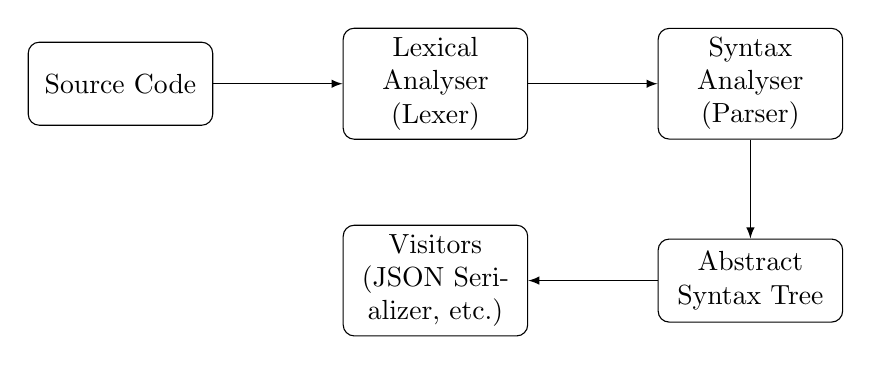
\begin{tikzpicture}[node distance=2cm, auto]
      % Define block styles
      \tikzstyle{block} = [rectangle, draw, text width=6em, text centered, rounded corners, minimum height=3em]
      \tikzstyle{line} = [draw, -latex]
      
      % Place blocks
      \node [block] (source) {Source Code};
      \node [block, right of=source, node distance=4cm] (lexer) {Lexical Analyser (Lexer)};
      \node [block, right of=lexer, node distance=4cm] (parser) {Syntax Analyser (Parser)};
      \node [block, below of=parser, node distance=2.5cm] (ast) {Abstract Syntax Tree};
      \node [block, left of=ast, node distance=4cm] (visitor) {Visitors (JSON Serializer, etc.)};
      
      % Draw lines
      \path [line] (source) -- (lexer);
      \path [line] (lexer) -- (parser);
      \path [line] (parser) -- (ast);
      \path [line] (ast) -- (visitor);
    \end{tikzpicture}
    \caption{High-level architecture of the \texttt{tinyC} compiler frontend}
    \label{fig:architecture}
\end{figure}

\pagebreak
The architecture consists of the following main components:

\begin{enumerate}
    \item \textbf{Lexical Analyser (Lexer)}: The lexer reads the source code character by character and groups them into tokens according to the lexical rules of \texttt{tinyC}. It handles whitespace, comments, and reports lexical errors.

    \item \textbf{Syntax Analyser (Parser)}: The parser takes the token stream produced by the lexer and verifies that it conforms to the \texttt{tinyC} grammar. It constructs an abstract syntax tree and reports syntax errors.

    \item \textbf{Abstract Syntax Tree (AST)}: The AST represents the hierarchical structure of the parsed program. Each node in the tree corresponds to a language construct in the source code.
    
    \item \textbf{Visitors}: The visitor pattern is implemented to traverse the AST for various operations. The most important visitor is the JSON serializer, which converts the AST to a standardized JSON representation. Other potential visitors could include a pretty-printer, static analyzer, or code generator.
\end{enumerate}

The core implementation is structured as a library (lib\texttt{tinyC}) that can be used directly in C++ projects. A separate command-line interface (\texttt{tinyC}-compiler) is built on top of this library, providing the standalone executable functionality.

\section{AST Design}

The AST design follows object-oriented principles to create a clear, maintainable, and extensible representation of \texttt{tinyC} programs. The design prioritizes simplicity, allowing students to easily work with the AST representation regardless of their implementation language.

\subsection{Node Structure}

The AST consists of various node types that represent different language constructs in \texttt{tinyC}. Rather than implementing a monolithic node class with numerous type-specific fields, the design employs a class hierarchy with a common base class (\texttt{ASTNode}) and specialized derived classes for different language elements. This approach follows the Single Responsibility Principle, with each class representing exactly one language construct.

Key node categories include declaration nodes for variables, functions, and structs; type nodes representing primitive types, named types, and pointer types; expression nodes for literals, identifiers, and operations; and statement nodes for blocks, conditionals, loops, and other control structures. Each node contains specific fields relevant to its language construct and provides access methods that expose these fields while maintaining appropriate encapsulation.

The base \texttt{ASTNode} class establishes common functionality across all nodes, including source location tracking for error reporting. Each derived class extends this base with construct-specific fields and behavior. This inheritance hierarchy allows for both static type safety through C++'s type system and runtime type identification through virtual functions and the visitor pattern.

\subsection{Memory Management}

The AST uses \texttt{std::unique\_ptr} for managing node ownership, a choice that naturally aligns with the hierarchical structure of abstract syntax trees. In an AST, each node has exactly one parent (except the root), creating a clear ownership hierarchy that unique pointers enforce at compile time. This approach offers several advantages over alternatives like \texttt{std::shared\_ptr}.

Unique pointers eliminate the reference counting overhead of shared pointers—an unnecessary cost for tree structures with clear parent-child relationships. They also prevent circular reference problems that could arise with shared pointers if the AST implementation needed cross-references between nodes. When using unique pointers, such relationships must be implemented as non-owning raw pointers, making ownership direction explicit and preventing accidental memory leaks.

From a design perspective, unique pointers make ownership transfer explicit through \texttt{std::move}, clearly indicating when a node becomes part of the parent structure. This explicitness improves code readability—particularly valuable in an educational context—while ensuring deterministic destruction that follows the tree hierarchy when nodes are deleted. This approach balances memory safety with performance considerations while maintaining a clear, understandable implementation.


\subsection{Visitor Pattern Implementation}

The visitor pattern provides a mechanism for performing operations on the AST without modifying the node classes, adhering to the Open-Closed Principle. This design pattern is particularly valuable in compiler construction, where different passes (e.g., semantic analysis, optimization, code generation) need to traverse the same AST structure while performing different operations.

The base \texttt{NodeVisitor} interface declares virtual \texttt{visit} methods for each concrete node type, as shown in Listing~\ref{code:node-visitor-interface}:

\begin{listing}[!h]
\begin{minted}{cpp}
class NodeVisitor {
public:
    virtual ~NodeVisitor() = default;
    
    // Visit methods for declaration nodes
    virtual void visit(const VariableNode& node) = 0;
    virtual void visit(const FunctionDeclarationNode& node) = 0;
    // ... other declarations
    
    // Visit methods for type nodes
    virtual void visit(const PrimitiveTypeNode& node) = 0;
    // ... other types
    
    // Visit methods for expression nodes
    virtual void visit(const LiteralNode& node) = 0;
    // ... other expressions
    
    // Visit methods for statement nodes
    virtual void visit(const BlockStatementNode& node) = 0;
    // ... other statements
};
\end{minted}
\caption{NodeVisitor interface declaration}
\label{code:node-visitor-interface}
\end{listing}

Each AST node implements an \texttt{accept} method that invokes the appropriate \texttt{visit} method on the visitor, as demonstrated in Listing~\ref{code:block-stmt-node-accept}:

\begin{listing}[ht!]
\begin{minted}{cpp}
void BlockStatementNode::accept(NodeVisitor& visitor) const {
    visitor.visit(*this);
}
\end{minted}
\caption{BlockStatementNode's accept method}
\label{code:block-stmt-node-accept}
\end{listing}

This design allows for adding new operations on the AST without modifying the node classes, adhering to the Open-Closed Principle as discussed in the visitor pattern implementation.



\subsection{Source Location Tracking}

Each AST node includes source location information to facilitate error reporting and debugging, as shown in Listing~\ref{code:ast-node-base-class}:

\begin{listing}[h!]
\begin{minted}{cpp}
class ASTNode {
public:
    explicit ASTNode(lexer::SourceLocation location);
    virtual ~ASTNode() = default;
    
    [[nodiscard]] lexer::SourceLocation getLocation() const;
    
    virtual void accept(NodeVisitor& visitor) const = 0;

private:
    const lexer::SourceLocation location;
};
\end{minted}
\caption{ASTNode base class declaration}
\label{code:ast-node-base-class}
\end{listing}

The \texttt{SourceLocation} struct contains the filename, line number (1-based), and column number (1-based). This information originates in the lexer, which tracks position as it tokenizes the source code. The parser then passes this location information to created AST nodes, ensuring that every node can be traced back to its origin in the source code.

This location tracking is particularly valuable for error reporting during later compilation phases. When a semantic error is detected (e.g., type mismatch or undeclared variable), the compiler can provide precise information about where the error occurred, greatly assisting students in debugging their \texttt{tinyC} programs.


\section{API Design}

The \texttt{tinyC} compiler frontend provides two main interfaces: a C++ library API for direct integration into student projects and a command-line interface for language-agnostic usage. This dual approach maximizes flexibility, accommodating students with varying programming language preferences and experience levels.


\subsection{Library API}

The library API allows direct integration of the \texttt{tinyC} frontend into C++ projects. This approach is ideal for students who prefer working in C++ and want tight integration between the frontend and their backend implementation. The API is designed with simplicity and clarity in mind, providing intuitive access to the frontend's core functionality.
The main entry point for lexical analysis is the \texttt{Lexer} class, shown in Listing~\ref{code:lexer-interface}:
\begin{listing}[ht!]
    \begin{minted}{cpp}
    namespace tinyC::lexer {
        class Lexer {
        public:
            explicit Lexer(std::string source, 
                           std::string filename = "<input>");
            TokenPtr nextToken();
            std::vector<TokenPtr> tokenize();
        };
    }
    \end{minted}
    \caption{Lexer class interface}
    \label{code:lexer-interface}
\end{listing}

The \texttt{Lexer} constructor accepts the source code as a string, along with an optional filename for error reporting. The \texttt{nextToken} method returns the next token in the input stream, while the \texttt{tokenize} method processes the entire input and returns a vector of all tokens. This design allows for both incremental token-by-token processing and batch processing of the entire input.

For syntax analysis, the \texttt{Parser} class provides the entry point, as shown in Listing~\ref{code:parser-interface}:

\begin{listing}[ht!]
\begin{minted}{cpp}
namespace tinyC::parser {
    class Parser {
    public:
        explicit Parser(lexer::Lexer& lexer);
        ast::ASTNodePtr parseProgram();
    };
}
\end{minted}
\caption{Parser class interface}
\label{code:parser-interface}
\end{listing}

The \texttt{Parser} constructor takes a reference to a \texttt{Lexer} instance, establishing the token source. The \texttt{parseProgram} method initiates parsing of the entire program, returning the root node of the resulting AST. This approach decouples the lexer and parser, allowing for separate testing and potential reuse of the lexer with different parsers.

For AST traversal and processing, the library provides visitor classes that implement the \texttt{NodeVisitor} interface, as shown in Listing~\ref{code:visitor-classes}:

\begin{listing}[ht!]
\begin{minted}{cpp}
namespace tinyC::ast {
    class DumpVisitor : public NodeVisitor {
    public:
        explicit DumpVisitor(std::ostream& os);
        // Visit methods for all node types
    };
    
    class JSONVisitor : public NodeVisitor {
    public:
        explicit JSONVisitor(bool prettyPrint = true);
        std::string getJSON() const;
        // Visit methods for all node types
    };
}
\end{minted}
\caption{Visitor classes for AST traversal}
\label{code:visitor-classes}
\end{listing}

The \texttt{DumpVisitor} outputs a human-readable representation of the AST to the specified output stream, useful for debugging and understanding the parsed structure. The \texttt{JSONVisitor} converts the AST to its JSON representation, with control over formatting through the \texttt{prettyPrint} option. The resulting JSON can be retrieved as a string using the \texttt{getJSON} method.

This API design prioritizes flexibility and ease of use. Students can work directly with the AST classes, implement their own visitors for custom operations, and control the parsing process step by step. The clear separation of concerns between lexical analysis, syntax analysis, and AST processing provides a solid foundation for understanding compiler structure.


\subsection{Command-Line Interface}

The command-line interface provides a standalone executable for parsing \texttt{tinyC} source files and outputting the AST as JSON. The main functionalities include:

\begin{enumerate}
    \item \textbf{Lexical Analysis Mode}: The command \texttt{tinyC-compiler --lex file.tc} tokenizes the input file and outputs the tokens. This mode is useful for debugging lexical issues and understanding how the source code is tokenized.

    \item \textbf{Parsing Mode}: The command \texttt{tinyC-compiler --parse file.tc} parses the input file and outputs the AST as JSON. This is the primary mode for students implementing their own backends, as it provides the complete AST structure in a standardized format.

    \item \textbf{Interactive Mode}: Running \texttt{tinyC-compiler} without arguments launches an interactive shell where students can enter \texttt{tinyC} code and immediately see the resulting tokens or AST. This mode is particularly useful for learning and experimentation.
\end{enumerate}

The command-line interface is designed to be simple and intuitive, with clear error messages and help text, making it accessible to students with varying levels of experience.

\subsection{JSON Output Format}
The JSON output format provides a standardized representation of the AST that can be consumed by any programming language. This format is the key to enabling language-agnostic backend implementation, as it decouples the frontend from any specific programming language or framework.

The JSON representation follows a well-defined schema with these key characteristics:

\begin{enumerate}
    \item \textbf{Node Type Identification}: Each node includes a \texttt{nodeType} field that identifies its type, allowing backends to process nodes according to their specific language construct.
    \item \textbf{Hierarchical Structure}: The JSON structure mirrors the hierarchical structure of the AST, with parent nodes containing their children as nested objects or arrays.
    \item \textbf{Source Locations}: Each node includes location information with filename, line, and column, enabling precise error reporting in later compilation phases.
    \item \textbf{Type-Specific Fields}: Each node type includes fields specific to that language construct, providing all necessary information for backend processing.
\end{enumerate}

An example JSON output for a simple variable declaration illustrating these characteristics is shown in Listing~\ref{code:json-example}.

\begin{listing}[h!]
\begin{minted}{json}
{
  "nodeType": "Program",
  "declarations": [
    {
      "nodeType": "VariableDeclaration",
      "identifier": "x",
      "type": {
        "nodeType": "PrimitiveType",
        "kind": "int",
        "location": {
          "filename": "example.tc",
          "line": 1,
          "column": 1
        }
      },
      "initializer": {
        "nodeType": "Literal",
        "kind": "integer",
        "value": "42",
        "location": {
          "filename": "example.tc",
          "line": 1,
          "column": 7
        }
      },
      "location": {
        "filename": "example.tc",
        "line": 1,
        "column": 5
      }
    }
  ],
  "location": {
    "filename": "example.tc",
    "line": 1,
    "column": 1
  }
}
\end{minted}
\caption{Example JSON output for a variable declaration: \texttt{int x = 42;}}
\label{code:json-example}
\end{listing}

This example demonstrates how the JSON format captures the hierarchical structure of the AST, with the program containing a variable declaration that includes a type and an initializer expression. Each node includes its type and location information, providing a complete representation of the parsed program.



% \pagebreak







\section{Test Suite Architecture}
The test suite for the \texttt{tinyC} compiler frontend is a comprehensive framework designed to validate the correctness of both the provided implementation and student-created alternatives. It offers systematic verification of lexical analysis, parsing functionality, and error handling capabilities.

\subsection{Test File Structure and Format}
The test files follow a metadata-driven format that allows precise specification of expected outcomes. Each test file contains:

\begin{listing}[h!]
\begin{minted}{text}
// tinyC TEST
// INFO: description of the test's purpose
// RUN: test type specification (parser, exec)
// EXPECT: expected outcome (SUCCESS, PARSER_ERROR, or LEXER_ERROR)
// RESULT: expected JSON output (for SUCCESS tests only)

// Actual TinyC code follows...
\end{minted}
\caption{Example test file structure showing the required metadata header}
\label{code:test-file-structure}
\end{listing}

This approach separates test expectations from the code being tested, making it easier to understand the purpose of each test and to verify correct functionality. The addition of the \texttt{RUN} directive enables the test framework to support different testing modes, particularly distinguishing between parser validation tests and execution tests that can be used once a backend implementation is available.

\subsection{Test Categories}
The test suite encompasses several categories of tests. The basic language feature tests cover empty programs, variable declarations and initializations, arrays and pointers, basic expressions and operations, and function declarations and definitions. Advanced language feature tests include control structures (if-else, loops, switch-case), struct declarations and usage, function pointers, type casting, and complex expressions with nested operations.

For error handling, the test suite verifies proper detection and reporting of lexical errors (such as invalid characters and unterminated strings/comments) and syntax errors (including mismatched parentheses and missing semicolons). Additionally, the test suite addresses edge cases by testing deeply nested expressions, complex combinations of language features, and boundary conditions for different constructs.

These comprehensive test categories ensure that the parser correctly handles the full spectrum of \texttt{tinyC} language features while providing appropriate error messages for invalid inputs.

\subsection{Test Runner Capabilities}
The \texttt{test\_runner.py} script executes and validates tests through several key features. It supports targeted testing through command-line options, allowing users to run individual tests by number (\texttt{--test} flag), a range of tests (\texttt{--range} flag), or all available tests by default.

For successful parses, the runner validates the JSON output against a formal schema specification, performs structural comparison between expected and actual AST structures, and uses semantic equivalence comparison rather than exact string matching. The runner handles source location information, which can vary but must follow the correct format.

When testing error conditions, the runner verifies that the appropriate error type is reported (lexical or syntax), checks for informative error messages, and validates that the parser exits with a non-zero code for errors. The test runner provides test-by-test reports showing pass/fail status, error diagnostics for failed tests, comparison of expected vs. actual outputs with previews, and summary statistics at the end.

\subsection{Schema Validation}
The test suite includes a formal JSON schema that defines the expected structure of the AST. This schema validates node types and required fields, ensures proper nesting of AST components, and verifies that source location information is present and properly formatted. As shown in Listing~\ref{code:json-schema-root}, the schema defines the root Program node structure with its required properties and references to other node definitions. The schema serves both as documentation of the JSON format and as a validation tool, ensuring that AST outputs conform to the expected structure. This is particularly valuable for students implementing their own parsers, as it provides immediate feedback about structural correctness.

\begin{listing}[ht]
\begin{minted}{json}
{
    "type": "object",
    "properties": {
        "nodeType": {
            "enum": ["Program"]
        },
        "declarations": {
            "type": "array",
            "items": {
                "oneOf": [
                    { "$ref": "#/definitions/VariableDeclaration" },
                    { "$ref": "#/definitions/FunctionDeclaration" },
                    { "$ref": "#/definitions/StructDeclaration" },
                    { "$ref": "#/definitions/FunctionPointerDeclaration" }
                ]
            }
        },
        "location": { "$ref": "#/definitions/SourceLocation" }
    },
    "required": ["nodeType", "declarations", "location"]
}
\end{minted}
\caption{Excerpt from the JSON schema showing the root Program node structure}
\label{code:json-schema-root}
\end{listing}

\subsection{Test Generation Utilities}
The \texttt{test\_generator.py} utility complements the test runner by automatically generating test files from example \texttt{tinyC} code. It creates expected JSON outputs for validation, maintains a consistent test nomenclature and organization, and supports different test categories with appropriate descriptions. The test generator provides a systematic way to create new tests as the implementation evolves, ensuring consistent test coverage across language features.

\subsection{Educational Value}
The test suite is designed with educational objectives in mind. Tests progressively introduce language features, helping students understand the language incrementally. The detailed error reporting guides students toward correct implementations, while the test framework itself demonstrates good testing practices. Students can extend the test suite with their own tests as they implement additional features, providing a practical way to learn about test-driven development and compiler construction.




\section{Summary}

This chapter has outlined the design requirements and architecture of the \texttt{tinyC} compiler frontend. The functional and non-functional requirements define what the system must accomplish and how it should behave. The \texttt{tinyC} grammar analysis identified key challenges and informed the parsing approach. The system architecture, AST design, API specifications, and test suite architecture collectively provide a comprehensive blueprint for an educational compiler frontend that meets the needs of NI-GEN course students.

The design emphasizes clarity, modularity, and educational value, enabling students to focus on compiler middle-end and back-end development while providing a solid foundation for understanding compiler frontends.

\chapter{Evaluation}

This chapter presents a concise evaluation of the \texttt{tinyC} compiler frontend developed in this thesis, focusing on its practical advantages and limitations within the educational context of the NI-GEN course.

\section{Comparison with Existing Implementation}

The current \texttt{tinyC} parser implementation provided to students in the NI-GEN course has several significant shortcomings that this project aims to address:

\begin{itemize}
    \item \textbf{Reliability Issues}: The existing implementation contains numerous bugs that require substantial debugging effort from students before they can even begin their backend work.
    
    \item \textbf{Inflexible Design}: Students are effectively forced to implement their backends in C++ regardless of their proficiency level, as the existing parser cannot easily output to a language-agnostic format.
    
    \item \textbf{Limited Documentation}: The existing implementation lacks documentation, making it difficult for students to understand the inner workings of the parser.
\end{itemize}

The \texttt{tinyC} compiler frontend developed in this thesis addresses these issues through its implementation, clear object-oriented design, test suite, and language-agnostic JSON output. The dual interface approach—providing both a C++ library and a standalone executable—gives students the flexibility to work in their preferred programming language without sacrificing quality or functionality.

\section{Functional Assessment}

The frontend successfully fulfills the key requirements outlined in Chapter 4:

\begin{itemize}
    \item The lexical analyzer correctly identifies all token types in the \texttt{tinyC} language, handling whitespace, comments, and reporting precise location information for errors.
    
    \item The syntax analyzer implements the LL(1) grammar and accurately constructs an AST that represents the program structure with clear error messages.
    
    \item The AST implementation follows object-oriented principles with a clean hierarchy of node types, and consistently tracks source location information.
    
    \item The JSON output follows a well-defined schema that includes all necessary information from the AST nodes and their source locations.
\end{itemize}

\section{Limitations}

Despite its improvements over the existing implementation, the frontend has certain limitations:

\begin{itemize}
    \item \textbf{Limited Error Recovery}: The parser stops after encountering the first syntax error rather than attempting to continue and identify multiple errors in a single pass.
    
    \item \textbf{No Student Feedback}: Unfortunately, due to timing constraints—this thesis being completed in the summer semester while the NI-GEN course runs in the winter semester—it has not been possible to gather direct feedback from students on the frontend's effectiveness in a real course setting.
    
    \item \textbf{Semantic Analysis Boundaries}: By design, the frontend does not perform semantic analysis tasks such as type checking or scope resolution, leaving these aspects for student implementation.
\end{itemize}


\section{Summary}

The evaluation indicates that the \texttt{tinyC} compiler frontend represents a significant improvement over the existing implementation provided to students. Its clean architecture, documentation, and dual interface approach make it well-suited for educational purposes, while its implementation and testing ensure reliability.

While direct student feedback is not yet available, the technical improvements and design considerations suggest that the frontend will effectively serve its primary goal of allowing students to focus on backend compiler development, providing a solid foundation for their coursework in the NI-GEN course.

% Conclusion
\chapter{Conclusion}

This thesis has presented the design and implementation of a compiler frontend for the \texttt{tinyC} programming language, specifically created for students of the NI-GEN course. The project aimed to provide students with a reliable parsing tool that would allow them to focus on the middle-end and back-end aspects of compiler construction, which are the main learning objectives of the course.

\section{Summary of Achievements}

The key achievements of this thesis include:

\begin{itemize}
    \item Development of a lexical analyzer capable of tokenizing \texttt{tinyC} source code with location tracking
    \item Implementation of a predictive recursive descent parser that handles the entire \texttt{tinyC} grammar and generates meaningful error messages
    \item Design of a clean, object-oriented abstract syntax tree structure with a visitor pattern implementation
    \item Creation of both a direct C++ library interface and a standardized JSON output format for language-agnostic consumption
    \item Implementation of a testing framework with metadata-driven test files, schema validation, and detailed error reporting
\end{itemize}

\section{Revisiting the Original Objectives}

The thesis set out to accomplish four main objectives, which have been successfully addressed:

\begin{enumerate}
    \item \textbf{Analyze the landscape of language parsers and language-agnostic AST representations}: Chapter 3 provided an analysis of existing parser technologies, AST designs, and serialization formats, forming the theoretical foundation for the implementation decisions.
    
    \item \textbf{Design and document AST representation for \texttt{tinyC} and its JSON format}: Chapter 4 detailed the AST hierarchy for \texttt{tinyC}, documenting both the internal class structure and the corresponding JSON schema.
    
    \item \textbf{Design, document, implement and test the \texttt{tinyC} parser}: Chapter 4 presented the design and implementation of the entire frontend, supported by an extensive test suite.
    
    \item \textbf{Discuss further development of the project}: The limitations and potential extensions have been discussed in Chapter 5 (Evaluation) and below in Future Work.
\end{enumerate}

\section{Limitations}

While the implemented frontend successfully meets its primary objectives, some limitations remain:

\begin{itemize}
    \item The error recovery mechanisms are relatively basic, stopping after the first syntax error rather than attempting to recover and continue parsing
    \item The frontend focuses exclusively on lexical and syntactic analysis, deliberately leaving semantic analysis for student implementation
\end{itemize}

These limitations are intentional boundaries that define where the frontend's responsibilities end and where student work on the compiler middle-end begins.

\section{Future Work}

Several potential enhancements could be considered for future development:

\begin{itemize}
    \item \textbf{Enhanced error recovery}: Implementing more sophisticated error recovery techniques would allow the parser to continue after encountering errors, providing more detailed feedback.
    
    \item \textbf{IDE integration}: Developing plugins for popular IDEs would provide syntax highlighting, code completion, and inline error reporting for \texttt{tinyC}.
    
    \item \textbf{Web-based interface}: Creating a web application that allows students to experiment with \texttt{tinyC} parsing would make the tool more accessible.
    
    \item \textbf{Language server protocol implementation}: Supporting LSP would enable integration with a wide range of editors and IDEs.
\end{itemize}

\section{Educational Value}

The clean, object-oriented design and well-documented API further enhance the educational value of the frontend, providing students with clear examples and patterns they can apply in their own work. The visitor pattern implementation, in particular, demonstrates an elegant solution to the problem of separating concerns in compiler design.

The testing suite represents an additional contribution beyond the core frontend implementation. It provides students with a systematic way to verify their own implementations through metadata-driven test files and schema validation. The test framework demonstrates good software engineering practices, including test-driven development, automated validation, and detailed error reporting. This extra work significantly enhances the educational value of the project by giving students both a reference implementation and a mechanism to validate their own work.

\section{Closing Remarks}

The \texttt{tinyC} compiler frontend developed in this thesis provides a solid foundation for students in the NI-GEN course to focus on the middle-end and back-end aspects of compiler construction. By offering both a direct C++ library interface and a language-agnostic JSON output format, it accommodates a variety of implementation approaches while maintaining a consistent representation of the \texttt{tinyC} language.

While there are opportunities for enhancement, the current implementation successfully fulfills its primary objective: providing a reliable, well-designed, and tested compiler frontend that allows students to focus on the core learning objectives of the NI-GEN course. The true measure of success will be seen when the frontend is deployed in future offerings of the course, potentially transforming the learning experience by enabling deeper exploration of optimization techniques and code generation strategies.


% Appendices
\appendix\appendixinit % do not remove these two commands



\section{Program and Program Items}
\begin{align*}
\text{PROGRAM}
  &\to \text{PROGRAM\_ITEM}\;\text{PROGRAM}\\
  &\to \varepsilon\\[6pt]
\text{PROGRAM\_ITEM}
  &\to \text{TYPE\_FUN\_RET}\;\text{identifier}\;\text{PROGRAM\_ITEM\_TAIL}\\
  &\to \text{STRUCT\_DECL}\\
  &\to \text{FUNPTR\_DECL}\\[6pt]
\text{PROGRAM\_ITEM\_TAIL}
  &\to (\,\text{OPT\_FUN\_ARGS}\,)\;\text{FUNC\_TAIL}\\
  &\to \text{GLOBAL\_VAR\_TAIL}\; ;\\[6pt]
\text{FUNC\_TAIL}
  &\to \text{BLOCK\_STMT}\\
  &\to ;
\end{align*}

\begin{align*}
\text{GLOBAL\_VAR\_TAIL}
  &\to \text{OPT\_ARRAY\_SIZE}\;\text{OPT\_INIT}\;\text{MORE\_GLOBAL\_VARS}\\[6pt]
\text{MORE\_GLOBAL\_VARS}
  &\to ,\;\text{identifier}\;\text{OPT\_ARRAY\_SIZE}\;\text{OPT\_INIT}\;\text{MORE\_GLOBAL\_VARS}\\
  &\to \varepsilon\\[6pt]
\text{OPT\_FUN\_ARGS}
  &\to \text{FUN\_ARG}\;\text{FUN\_ARG\_TAIL}\\
  &\to \varepsilon\\[6pt]
\text{FUN\_ARG\_TAIL}
  &\to ,\;\text{FUN\_ARG}\;\text{FUN\_ARG\_TAIL}\\
  &\to \varepsilon\\[6pt]
\text{FUN\_ARG}
  &\to \text{TYPE}\;\text{identifier}
\end{align*}

%----------------------------------------
\section{Statements}
\begin{align*}
\text{STATEMENT}
  &\to \text{BLOCK\_STMT}\\
  &\to \text{IF\_STMT}\\
  &\to \text{SWITCH\_STMT}\\
  &\to \text{WHILE\_STMT}\\
  &\to \text{DO\_WHILE\_STMT}\\
  &\to \text{FOR\_STMT}\\
  &\to \text{BREAK\_STMT}\\
  &\to \text{CONTINUE\_STMT}\\
  &\to \text{RETURN\_STMT}\\
  &\to \text{EXPR\_STMT}\\[6pt]
\text{BLOCK\_STMT}
  &\to \{\,\text{STATEMENT\_STAR}\,\}\\[6pt]
\text{STATEMENT\_STAR}
  &\to \text{STATEMENT}\;\text{STATEMENT\_STAR}\\
  &\to \varepsilon
\end{align*}

\begin{align*}
\text{IF\_STMT}
  &\to \text{if}\;(\,\text{EXPR}\,)\;\{\,\text{STATEMENT}\}\;\text{ELSE\_PART}\\[6pt]
\text{ELSE\_PART}
  &\to \text{else}\;\text{STATEMENT}\\
  &\to \varepsilon\\[6pt]
\text{SWITCH\_STMT}
  &\to \text{switch}\;(\,\text{EXPR}\,)\;\{\,\text{CASE\_WITH\_DEFAULT\_STMT\_STAR}\}\\[6pt]
\text{CASE\_WITH\_DEFAULT\_STMT\_STAR}
  &\to \text{CASE\_STMT}\;\text{CASE\_WITH\_DEFAULT\_STMT\_STAR}\\
  &\to \varepsilon\\
  &\to \text{DEFAULT\_CASE}\;\text{CASE\_STMT\_STAR}\\[6pt]
\text{CASE\_STMT\_STAR}
  &\to \text{CASE\_STMT}\;\text{CASE\_STMT\_STAR}\\
  &\to \varepsilon\\[6pt]
\text{CASE\_STMT}
  &\to \text{case}\;\text{integer\_literal}\;:\;\text{CASE\_BODY}\\[6pt]
\text{CASE\_BODY}
  &\to \text{STATEMENT\_STAR}\\[6pt]
\text{DEFAULT\_CASE}
  &\to \text{default}\;:\;\text{CASE\_BODY}
\end{align*}

\begin{align*}
\text{WHILE\_STMT}
  &\to \text{while}\;(\,\text{EXPR}\,)\;\text{STATEMENT}\\[6pt]
\text{DO\_WHILE\_STMT}
  &\to \text{do}\;\text{STATEMENT}\;\text{while}\;(\,\text{EXPR}\,)\; ;\\[6pt]
\text{FOR\_STMT}
  &\to \text{for}\;( \text{OPT\_EXPR\_OR\_VAR\_DECL}\; ;\; \text{OPT\_EXPR}\; ;\; \text{OPT\_EXPR} )\;\text{STATEMENT}\\[6pt]
\text{OPT\_EXPR\_OR\_VAR\_DECL}
  &\to \text{EXPR\_OR\_VAR\_DECL}\\
  &\to \varepsilon\\[6pt]
\text{OPT\_EXPR}
  &\to \text{EXPR}\\
  &\to \varepsilon
\end{align*}

\begin{align*}
\text{BREAK\_STMT}
  &\to \text{break}\; ;\\[6pt]
\text{CONTINUE\_STMT}
  &\to \text{continue}\; ;\\[6pt]
\text{RETURN\_STMT}
  &\to \text{return}\;\text{OPT\_EXPR}\; ;\\[6pt]
\text{EXPR\_STMT}
  &\to \text{EXPR\_OR\_VAR\_DECL}\; ;
\end{align*}

%----------------------------------------
\section{Expression or Variable Declarations}
\begin{align*}
\text{EXPR\_OR\_VAR\_DECL}
  &\to \text{VAR\_DECLS}\\
  &\to \text{EXPRS}\\[6pt]
\text{VAR\_DECLS}
  &\to \text{VAR\_DECL}\;\text{VAR\_DECLS\_TAIL}\\[6pt]
\text{VAR\_DECLS\_TAIL}
  &\to ,\;\text{VAR\_DECL}\;\text{VAR\_DECLS\_TAIL}\\
  &\to \varepsilon\\[6pt]
\text{VAR\_DECL}
  &\to \text{TYPE}\;\text{identifier}\;\text{OPT\_ARRAY\_SIZE}\;\text{OPT\_INIT}\\[6pt]
\text{OPT\_ARRAY\_SIZE}
  &\to [\;\text{E9}\;]\\
  &\to \varepsilon\\[6pt]
\text{OPT\_INIT}
  &\to =\;\text{EXPR}\\
  &\to \varepsilon
\end{align*}

\begin{align*}
\text{EXPRS}
  &\to \text{EXPR}\;\text{EXPRS\_TAIL}\\[6pt]
\text{EXPRS\_TAIL}
  &\to ,\;\text{EXPR}\;\text{EXPRS\_TAIL}\\
  &\to \varepsilon
\end{align*}

%----------------------------------------
\section{Types}
\begin{align*}
\text{TYPE\_FUN\_RET}
  &\to \text{BaseOrIdType}\\
  &\to \text{void}\;\text{TypeFunRetTail}\\[6pt]
\text{BaseOrIdType}
  &\to \text{BASE\_TYPE}\;\text{STAR\_SEQ}\\
  &\to \text{TYPENAME}\;\text{STAR\_SEQ}\\[6pt]
\text{TypeFunRetTail}
  &\to \text{STAR\_PLUS}\\
  &\to \varepsilon\\[6pt]
\text{TYPE}
  &\to \text{BaseOrIdType}\\
  &\to \text{void}\;\text{STAR\_PLUS}\\[6pt]
\text{BASE\_TYPE}
  &\to \text{int}\\
  &\to \text{double}\\
  &\to \text{char}\\[6pt]
\text{STAR\_PLUS}
  &\to *\;\text{STAR\_SEQ}\\[6pt]
\text{STAR\_SEQ}
  &\to *\;\text{STAR\_SEQ}\\
  &\to \varepsilon
\end{align*}

%----------------------------------------
\section{Struct Declarations}
\begin{align*}
\text{STRUCT\_DECL}
  &\to \text{struct}\;\text{identifier}\;\text{OPT\_STRUCT\_BODY}\; ;\\[6pt]
\text{OPT\_STRUCT\_BODY}
  &\to \{\,\text{STRUCT\_FIELDS}\,\}\\
  &\to \varepsilon\\[6pt]
\text{STRUCT\_FIELDS}
  &\to \text{STRUCT\_FIELD}\;\text{STRUCT\_FIELDS}\\
  &\to \varepsilon\\[6pt]
\text{STRUCT\_FIELD}
  &\to \text{TYPE}\;\text{identifier}\; ;
\end{align*}

%----------------------------------------
\section{Function Pointer Declarations}
\begin{align*}
\text{FUNPTR\_DECL}
  &\to \text{typedef}\;\text{TYPE\_FUN\_RET}\;( *\;\text{identifier} )(\,\text{OPT\_FUNPTR\_ARGS}\,)\; ;\\[6pt]
\text{OPT\_FUNPTR\_ARGS}
  &\to \text{FUNPTR\_ARGS}\\
  &\to \varepsilon\\[6pt]
\text{FUNPTR\_ARGS}
  &\to \text{TYPE}\;\text{FUNPTR\_ARGS\_TAIL}\\[6pt]
\text{FUNPTR\_ARGS\_TAIL}
  &\to ,\;\text{TYPE}\;\text{FUNPTR\_ARGS\_TAIL}\\
  &\to \varepsilon
\end{align*}

%----------------------------------------
\section{Expressions}
\begin{align*}
\text{EXPR}
  &\to \text{E9}\;\text{EXPR\_TAIL}\\[6pt]
\text{EXPR\_TAIL}
  &\to =\;\text{EXPR}\\
  &\to \varepsilon
\end{align*}

\begin{align*}
\text{E9}
  &\to \text{E8}\;\text{E9\_Prime}\\[6pt]
\text{E9\_Prime}
  &\to ||\;\text{E8}\;\text{E9\_Prime}\\
  &\to \varepsilon
\end{align*}

\begin{align*}
\text{E8}
  &\to \text{E7}\;\text{E8\_Prime}\\[6pt]
\text{E8\_Prime}
  &\to &&\;\text{E7}\;\text{E8\_Prime}\\
  &\to \varepsilon
\end{align*}

\begin{align*}
\text{E7}
  &\to \text{E6}\;\text{E7\_Prime}\\[6pt]
\text{E7\_Prime}
  &\to |\;\text{E6}\;\text{E7\_Prime}\\
  &\to \varepsilon
\end{align*}

\begin{align*}
\text{E6}
  &\to \text{E5}\;\text{E6\_Prime}\\[6pt]
\text{E6\_Prime}
  &\to &\;\text{E5}\;\text{E6\_Prime}\\
  &\to \varepsilon
\end{align*}

\begin{align*}
\text{E5}
  &\to \text{E4}\;\text{E5\_Prime}\\[6pt]
\text{E5\_Prime}
  &\to ==\;\text{E4}\;\text{E5\_Prime}\\
  &\to !=\;\text{E4}\;\text{E5\_Prime}\\
  &\to \varepsilon
\end{align*}

\begin{align*}
\text{E4}
  &\to \text{E3}\;\text{E4\_Prime}\\[6pt]
\text{E4\_Prime}
  &\to <\;\text{E3}\;\text{E4\_Prime}\\
  &\to <=\;\text{E3}\;\text{E4\_Prime}\\
  &\to >\;\text{E3}\;\text{E4\_Prime}\\
  &\to >=\;\text{E3}\;\text{E4\_Prime}\\
  &\to \varepsilon
\end{align*}

\begin{align*}
\text{E3}
  &\to \text{E2}\;\text{E3\_Prime}\\[6pt]
\text{E3\_Prime}
  &\to <<\;\text{E2}\;\text{E3\_Prime}\\
  &\to >>\;\text{E2}\;\text{E3\_Prime}\\
  &\to \varepsilon
\end{align*}

\begin{align*}
\text{E2}
  &\to \text{E1}\;\text{E2\_Prime}\\[6pt]
\text{E2\_Prime}
  &\to +\;\text{E1}\;\text{E2\_Prime}\\
  &\to -\;\text{E1}\;\text{E2\_Prime}\\
  &\to \varepsilon
\end{align*}

\begin{align*}
\text{E1}
  &\to \text{E\_UNARY\_PRE}\;\text{E1\_Prime}\\[6pt]
\text{E1\_Prime}
  &\to *\;\text{E\_UNARY\_PRE}\;\text{E1\_Prime}\\
  &\to /\;\text{E\_UNARY\_PRE}\;\text{E1\_Prime}\\
  &\to %\;\text{E\_UNARY\_PRE}\;\text{E1\_Prime}\\
  &\to \varepsilon
\end{align*}

\begin{align*}
\text{E\_UNARY\_PRE}
  &\to +\;\text{E\_UNARY\_PRE}\\
  &\to -\;\text{E\_UNARY\_PRE}\\
  &\to !\;\text{E\_UNARY\_PRE}\\
  &\to \sim\;\text{E\_UNARY\_PRE}\\
  &\to ++\;\text{E\_UNARY\_PRE}\\
  &\to --\;\text{E\_UNARY\_PRE}\\
  &\to *\;\text{E\_UNARY\_PRE}\\
  &\to &\;\text{E\_UNARY\_PRE}\\
  &\to \text{E\_CALL\_INDEX\_MEMBER\_POST}
\end{align*}

\begin{align*}
\text{E\_CALL\_INDEX\_MEMBER\_POST}
  &\to \text{F}\;\text{E\_CALL\_INDEX\_MEMBER\_POST\_Prime}\\[6pt]
\text{E\_CALL\_INDEX\_MEMBER\_POST\_Prime}
  &\to \text{E\_CALL}\;\text{E\_CALL\_INDEX\_MEMBER\_POST\_Prime}\\
  &\to \text{E\_INDEX}\;\text{E\_CALL\_INDEX\_MEMBER\_POST\_Prime}\\
  &\to \text{E\_MEMBER}\;\text{E\_CALL\_INDEX\_MEMBER\_POST\_Prime}\\
  &\to \text{E\_POST}\;\text{E\_CALL\_INDEX\_MEMBER\_POST\_Prime}\\
  &\to \varepsilon
\end{align*}

\begin{align*}
\text{E\_CALL}
  &\to (\;\text{OPT\_EXPR\_LIST}\;)\\[6pt]
\text{OPT\_EXPR\_LIST}
  &\to \text{EXPR}\;\text{EXPR\_TAIL\_LIST}\\
  &\to \varepsilon\\[6pt]
\text{EXPR\_TAIL\_LIST}
  &\to ,\;\text{EXPR}\;\text{EXPR\_TAIL\_LIST}\\
  &\to \varepsilon
\end{align*}

\begin{align*}
\text{E\_INDEX}
  &\to [\;\text{EXPR}\;]\\[6pt]
\text{E\_MEMBER}
  &\to .\;\text{identifier}\\
  &\to \sim>\;\text{identifier}\\[6pt]
\text{E\_POST}
  &\to ++\\
  &\to --
\end{align*}

\begin{align*}
\text{F}
  &\to \text{integer\_literal}\\
  &\to \text{double\_literal}\\
  &\to \text{char\_literal}\\
  &\to \text{string\_literal}\\
  &\to \text{identifier}\\
  &\to (\;\text{EXPR}\;)\\
  &\to \text{E\_CAST}\\[6pt]
\text{E\_CAST}
  &\to \text{cast}\;<\;\text{TYPE}\;>\;(\;\text{EXPR}\;)
\end{align*}

% \chapter{JSON Schema}
\label{appendix-b}
This appendix provides the complete JSON Schema definition for the \texttt{tinyC} Abstract Syntax Tree (AST). This schema formally defines the structure, properties, and constraints for all node types in the AST, ensuring consistent JSON serialization across different implementations.
The schema follows the JSON Schema specification (Draft-07) and can be used to validate AST outputs from any parser implementation. It defines the hierarchical structure of the \texttt{tinyC} language including expressions, statements, declarations, and types.




% Include the JSON schema
\begin{lstlisting}
{
    "$schema": "http://json-schema.org/draft-07/schema#",
    "title": "TinyC AST JSON Schema",
    "description": "JSON Schema for the AST representation of the TinyC language",
    "definitions": {
        "SourceLocation": {
        "type": "object",
        "required": [
            "filename",
            "line",
            "column"
        ],
        "properties": {
            "filename": {
            "type": "string",
            "description": "Source file name"
            },
            "line": {
            "type": "integer",
            "description": "Line number (1-based, 0 for whole file)"
            },
            "column": {
            "type": "integer",
            "description": "Column number (1-based, 0 for whole file)"
            }
        }
        },
        "Node": {
        "type": "object",
        "required": [
            "nodeType",
            "location"
        ],
        "properties": {
            "nodeType": {
            "type": "string",
            "description": "Type of the AST node"
            },
            "location": {
            "$ref": "#/definitions/SourceLocation"
            }
        }
        },
        "Expression": {
        "allOf": [
            {
            "$ref": "#/definitions/Node"
            }
        ]
        },
        "Statement": {
        "allOf": [
            {
            "$ref": "#/definitions/Node"
            }
        ]
        },
        "Declaration": {
        "allOf": [
            {
            "$ref": "#/definitions/Node"
            }
        ]
        },
        "Type": {
        "allOf": [
            {
            "$ref": "#/definitions/Node"
            }
        ]
        },
        "PrimitiveType": {
        "allOf": [
            {
            "$ref": "#/definitions/Type"
            },
            {
            "properties": {
                "nodeType": {
                "enum": [
                    "PrimitiveType"
                ]
                },
                "kind": {
                "type": "string",
                "enum": [
                    "int",
                    "double",
                    "char",
                    "void"
                ],
                "description": "Kind of primitive type"
                }
            },
            "required": [
                "kind"
            ]
            }
        ]
        },
        "NamedType": {
        "allOf": [
            {
            "$ref": "#/definitions/Type"
            },
            {
            "properties": {
                "nodeType": {
                "enum": [
                    "NamedType"
                ]
                },
                "identifier": {
                "type": "string",
                "description": "Name of the type (struct or typedef)"
                }
            },
            "required": [
                "identifier"
            ]
            }
        ]
        },
        "PointerType": {
        "allOf": [
            {
            "$ref": "#/definitions/Type"
            },
            {
            "properties": {
                "nodeType": {
                "enum": [
                    "PointerType"
                ]
                },
                "baseType": {
                "$ref": "#/definitions/Type",
                "description": "Base type of the pointer"
                }
            },
            "required": [
                "baseType"
            ]
            }
        ]
        },
        "Literal": {
        "allOf": [
            {
            "$ref": "#/definitions/Expression"
            },
            {
            "properties": {
                "nodeType": {
                "enum": [
                    "Literal"
                ]
                },
                "kind": {
                "type": "string",
                "enum": [
                    "integer",
                    "double",
                    "char",
                    "string"
                ],
                "description": "Kind of literal"
                },
                "value": {
                "oneOf": [
                    {
                    "type": "string"
                    },
                    {
                    "type": "number"
                    }
                ],
                "description": "Literal value (string for text, number for numeric literals)"
                }
            },
            "required": [
                "kind",
                "value"
            ]
            }
        ]
        },
        "Identifier": {
        "allOf": [
            {
            "$ref": "#/definitions/Expression"
            },
            {
            "properties": {
                "nodeType": {
                "enum": [
                    "Identifier"
                ]
                },
                "identifier": {
                "type": "string",
                "description": "Name of the identifier"
                }
            },
            "required": [
                "identifier"
            ]
            }
        ]
        },
        "BinaryExpression": {
        "allOf": [
            {
            "$ref": "#/definitions/Expression"
            },
            {
            "properties": {
                "nodeType": {
                "enum": [
                    "BinaryExpression"
                ]
                },
                "operator": {
                "type": "string",
                "description": "Binary operator (+, -, *, /, etc.)"
                },
                "left": {
                "$ref": "#/definitions/Expression",
                "description": "Left operand"
                },
                "right": {
                "$ref": "#/definitions/Expression",
                "description": "Right operand"
                }
            },
            "required": [
                "operator",
                "left",
                "right"
            ]
            }
        ]
        },
        "UnaryExpression": {
        "allOf": [
            {
            "$ref": "#/definitions/Expression"
            },
            {
            "properties": {
                "nodeType": {
                "enum": [
                    "UnaryExpression"
                ]
                },
                "operator": {
                "type": "string",
                "description": "Unary operator (+, -, !, ~, ++, --, *, &)"
                },
                "prefix": {
                "type": "string",
                "enum": [
                    "true",
                    "false"
                ],
                "description": "Whether the operator is prefix (true) or postfix (false)"
                },
                "operand": {
                "$ref": "#/definitions/Expression",
                "description": "Operand of the unary expression"
                }
            },
            "required": [
                "operator",
                "prefix",
                "operand"
            ]
            }
        ]
        },
        "CastExpression": {
        "allOf": [
            {
            "$ref": "#/definitions/Expression"
            },
            {
            "properties": {
                "nodeType": {
                "enum": [
                    "CastExpression"
                ]
                },
                "targetType": {
                "$ref": "#/definitions/Type",
                "description": "Type to cast to"
                },
                "expression": {
                "$ref": "#/definitions/Expression",
                "description": "Expression to cast"
                }
            },
            "required": [
                "targetType",
                "expression"
            ]
            }
        ]
        },
        "CallExpression": {
        "allOf": [
            {
            "$ref": "#/definitions/Expression"
            },
            {
            "properties": {
                "nodeType": {
                "enum": [
                    "CallExpression"
                ]
                },
                "callee": {
                "$ref": "#/definitions/Expression",
                "description": "Function to call"
                },
                "arguments": {
                "type": "array",
                "items": {
                    "$ref": "#/definitions/Expression"
                },
                "description": "Arguments for the function call"
                }
            },
            "required": [
                "callee",
                "arguments"
            ]
            }
        ]
        },
        "IndexExpression": {
        "allOf": [
            {
            "$ref": "#/definitions/Expression"
            },
            {
            "properties": {
                "nodeType": {
                "enum": [
                    "IndexExpression"
                ]
                },
                "array": {
                "$ref": "#/definitions/Expression",
                "description": "Array or pointer to index"
                },
                "index": {
                "$ref": "#/definitions/Expression",
                "description": "Index expression"
                }
            },
            "required": [
                "array",
                "index"
            ]
            }
        ]
        },
        "MemberExpression": {
        "allOf": [
            {
            "$ref": "#/definitions/Expression"
            },
            {
            "properties": {
                "nodeType": {
                "enum": [
                    "MemberExpression"
                ]
                },
                "kind": {
                "type": "string",
                "enum": [
                    "dot",
                    "arrow"
                ],
                "description": "Kind of member access (dot for struct, arrow for pointer to struct)"
                },
                "object": {
                "$ref": "#/definitions/Expression",
                "description": "Object to access"
                },
                "member": {
                "type": "string",
                "description": "Name of the member to access"
                }
            },
            "required": [
                "kind",
                "object",
                "member"
            ]
            }
        ]
        },
        "CommaExpression": {
        "allOf": [
            {
            "$ref": "#/definitions/Expression"
            },
            {
            "properties": {
                "nodeType": {
                "enum": [
                    "CommaExpression"
                ]
                },
                "expressions": {
                "type": "array",
                "items": {
                    "$ref": "#/definitions/Expression"
                },
                "description": "List of expressions separated by commas"
                }
            },
            "required": [
                "expressions"
            ]
            }
        ]
        },
        "BlockStatement": {
        "allOf": [
            {
            "$ref": "#/definitions/Statement"
            },
            {
            "properties": {
                "nodeType": {
                "enum": [
                    "BlockStatement"
                ]
                },
                "statements": {
                "type": "array",
                "items": {
                    "$ref": "#/definitions/Statement"
                },
                "description": "List of statements in the block"
                }
            },
            "required": [
                "statements"
            ]
            }
        ]
        },
        "ExpressionStatement": {
        "allOf": [
            {
            "$ref": "#/definitions/Statement"
            },
            {
            "properties": {
                "nodeType": {
                "enum": [
                    "ExpressionStatement"
                ]
                },
                "expression": {
                "$ref": "#/definitions/Expression",
                "description": "Expression to execute as a statement"
                }
            },
            "required": [
                "expression"
            ]
            }
        ]
        },
        "IfStatement": {
        "allOf": [
            {
            "$ref": "#/definitions/Statement"
            },
            {
            "properties": {
                "nodeType": {
                "enum": [
                    "IfStatement"
                ]
                },
                "condition": {
                "$ref": "#/definitions/Expression",
                "description": "Condition to check"
                },
                "thenBranch": {
                "$ref": "#/definitions/Statement",
                "description": "Statement to execute if condition is true"
                },
                "elseBranch": {
                "oneOf": [
                    {
                    "$ref": "#/definitions/Statement"
                    },
                    {
                    "type": "null"
                    }
                ],
                "description": "Statement to execute if condition is false (optional)"
                }
            },
            "required": [
                "condition",
                "thenBranch"
            ]
            }
        ]
        },
        "WhileStatement": {
        "allOf": [
            {
            "$ref": "#/definitions/Statement"
            },
            {
            "properties": {
                "nodeType": {
                "enum": [
                    "WhileStatement"
                ]
                },
                "condition": {
                "$ref": "#/definitions/Expression",
                "description": "Condition to check before each iteration"
                },
                "body": {
                "$ref": "#/definitions/Statement",
                "description": "Statement to execute in each iteration"
                }
            },
            "required": [
                "condition",
                "body"
            ]
            }
        ]
        },
        "DoWhileStatement": {
        "allOf": [
            {
            "$ref": "#/definitions/Statement"
            },
            {
            "properties": {
                "nodeType": {
                "enum": [
                    "DoWhileStatement"
                ]
                },
                "body": {
                "$ref": "#/definitions/Statement",
                "description": "Statement to execute in each iteration"
                },
                "condition": {
                "$ref": "#/definitions/Expression",
                "description": "Condition to check after each iteration"
                }
            },
            "required": [
                "body",
                "condition"
            ]
            }
        ]
        },
        "ForStatement": {
        "allOf": [
            {
            "$ref": "#/definitions/Statement"
            },
            {
            "properties": {
                "nodeType": {
                "enum": [
                    "ForStatement"
                ]
                },
                "initialization": {
                "oneOf": [
                    {
                    "$ref": "#/definitions/Expression"
                    },
                    {
                    "$ref": "#/definitions/Declaration"
                    },
                    {
                    "$ref": "#/definitions/MultipleDeclaration"
                    },
                    {
                    "type": "null"
                    }
                ],
                "description": "Initialization expression or variable declaration (optional)"
                },
                "condition": {
                "oneOf": [
                    {
                    "$ref": "#/definitions/Expression"
                    },
                    {
                    "type": "null"
                    }
                ],
                "description": "Condition to check before each iteration (optional)"
                },
                "update": {
                "oneOf": [
                    {
                    "$ref": "#/definitions/Expression"
                    },
                    {
                    "type": "null"
                    }
                ],
                "description": "Update expression to execute after each iteration (optional)"
                },
                "body": {
                "$ref": "#/definitions/Statement",
                "description": "Statement to execute in each iteration"
                }
            },
            "required": [
                "body"
            ]
            }
        ]
        },
        "SwitchCase": {
        "type": "object",
        "properties": {
            "isDefault": {
            "type": "boolean",
            "description": "Whether this is a default case or not"
            },
            "value": {
            "type": "integer",
            "description": "Case value (only for non-default cases)"
            },
            "body": {
            "type": "array",
            "items": {
                "$ref": "#/definitions/Statement"
            },
            "description": "List of statements in the case body"
            }
        },
        "required": [
            "isDefault",
            "body"
        ],
        "if": {
            "properties": {
            "isDefault": {
                "enum": [
                false
                ]
            }
            }
        },
        "then": {
            "required": [
            "value"
            ]
        }
        },
        "SwitchStatement": {
        "allOf": [
            {
            "$ref": "#/definitions/Statement"
            },
            {
            "properties": {
                "nodeType": {
                "enum": [
                    "SwitchStatement"
                ]
                },
                "expression": {
                "$ref": "#/definitions/Expression",
                "description": "Expression to switch on"
                },
                "cases": {
                "type": "array",
                "items": {
                    "$ref": "#/definitions/SwitchCase"
                },
                "description": "List of case clauses"
                }
            },
            "required": [
                "expression",
                "cases"
            ]
            }
        ]
        },
        "BreakStatement": {
        "allOf": [
            {
            "$ref": "#/definitions/Statement"
            },
            {
            "properties": {
                "nodeType": {
                "enum": [
                    "BreakStatement"
                ]
                }
            }
            }
        ]
        },
        "ContinueStatement": {
        "allOf": [
            {
            "$ref": "#/definitions/Statement"
            },
            {
            "properties": {
                "nodeType": {
                "enum": [
                    "ContinueStatement"
                ]
                }
            }
            }
        ]
        },
        "ReturnStatement": {
        "allOf": [
            {
            "$ref": "#/definitions/Statement"
            },
            {
            "properties": {
                "nodeType": {
                "enum": [
                    "ReturnStatement"
                ]
                },
                "expression": {
                "oneOf": [
                    {
                    "$ref": "#/definitions/Expression"
                    },
                    {
                    "type": "null"
                    }
                ],
                "description": "Return value (optional for void functions)"
                }
            }
            }
        ]
        },
        "VariableDeclaration": {
        "allOf": [
            {
            "$ref": "#/definitions/Declaration"
            },
            {
            "properties": {
                "nodeType": {
                "enum": [
                    "VariableDeclaration"
                ]
                },
                "identifier": {
                "type": "string",
                "description": "Name of the variable"
                },
                "type": {
                "$ref": "#/definitions/Type",
                "description": "Type of the variable"
                },
                "arraySize": {
                "oneOf": [
                    {
                    "$ref": "#/definitions/Expression"
                    },
                    {
                    "type": "null"
                    }
                ],
                "description": "Size of the array (optional, null for non-array variables)"
                },
                "initializer": {
                "oneOf": [
                    {
                    "$ref": "#/definitions/Expression"
                    },
                    {
                    "type": "null"
                    }
                ],
                "description": "Initial value (optional)"
                }
            },
            "required": [
                "identifier",
                "type"
            ]
            }
        ]
        },
        "MultipleDeclaration": {
        "allOf": [
            {
            "$ref": "#/definitions/Declaration"
            },
            {
            "properties": {
                "nodeType": {
                "enum": [
                    "MultipleDeclaration"
                ]
                },
                "declarations": {
                "type": "array",
                "items": {
                    "$ref": "#/definitions/VariableDeclaration"
                },
                "description": "List of variable declarations that share the same statement"
                }
            },
            "required": [
                "declarations"
            ]
            }
        ]
        },
        "Parameter": {
        "allOf": [
            {
            "$ref": "#/definitions/Declaration"
            },
            {
            "properties": {
                "nodeType": {
                "enum": [
                    "Parameter"
                ]
                },
                "identifier": {
                "type": "string",
                "description": "Name of the parameter"
                },
                "type": {
                "$ref": "#/definitions/Type",
                "description": "Type of the parameter"
                }
            },
            "required": [
                "identifier",
                "type"
            ]
            }
        ]
        },
        "FunctionDeclaration": {
        "allOf": [
            {
            "$ref": "#/definitions/Declaration"
            },
            {
            "properties": {
                "nodeType": {
                "enum": [
                    "FunctionDeclaration",
                    "FunctionDefinition"
                ]
                },
                "identifier": {
                "type": "string",
                "description": "Name of the function"
                },
                "returnType": {
                "$ref": "#/definitions/Type",
                "description": "Return type of the function"
                },
                "parameters": {
                "type": "array",
                "items": {
                    "$ref": "#/definitions/Parameter"
                },
                "description": "Function parameters"
                },
                "body": {
                "oneOf": [
                    {
                    "$ref": "#/definitions/BlockStatement"
                    },
                    {
                    "type": "null"
                    }
                ],
                "description": "Function body (null for declarations, BlockStatement for definitions)"
                }
            },
            "required": [
                "identifier",
                "returnType",
                "parameters"
            ]
            }
        ]
        },
        "StructDeclaration": {
        "allOf": [
            {
            "$ref": "#/definitions/Declaration"
            },
            {
            "properties": {
                "nodeType": {
                "enum": [
                    "StructDeclaration",
                    "StructDefinition"
                ]
                },
                "identifier": {
                "type": "string",
                "description": "Name of the struct"
                },
                "fields": {
                "type": "array",
                "items": {
                    "$ref": "#/definitions/VariableDeclaration"
                },
                "description": "Struct fields (empty for forward declarations)"
                }
            },
            "required": [
                "identifier",
                "fields"
            ]
            }
        ]
        },
        "FunctionPointerDeclaration": {
        "allOf": [
            {
            "$ref": "#/definitions/Declaration"
            },
            {
            "properties": {
                "nodeType": {
                "enum": [
                    "FunctionPointerDeclaration"
                ]
                },
                "identifier": {
                "type": "string",
                "description": "Name of the function pointer type"
                },
                "returnType": {
                "$ref": "#/definitions/Type",
                "description": "Return type of the function pointer"
                },
                "parameterTypes": {
                "type": "array",
                "items": {
                    "$ref": "#/definitions/Type"
                },
                "description": "Types of the function parameters"
                }
            },
            "required": [
                "identifier",
                "returnType",
                "parameterTypes"
            ]
            }
        ]
        }
    },
    "type": "object",
    "properties": {
        "nodeType": {
        "enum": [
            "Program"
        ]
        },
        "location": {
        "$ref": "#/definitions/SourceLocation"
        },
        "declarations": {
        "type": "array",
        "items": {
            "oneOf": [
            {
                "$ref": "#/definitions/VariableDeclaration"
            },
            {
                "$ref": "#/definitions/FunctionDeclaration"
            },
            {
                "$ref": "#/definitions/StructDeclaration"
            },
            {
                "$ref": "#/definitions/FunctionPointerDeclaration"
            },
            {
                "$ref": "#/definitions/MultipleDeclaration"
            }
            ]
        },
        "description": "Top-level declarations in the program"
        }
    },
    "required": [
        "nodeType",
        "location",
        "declarations"
    ]
}
\end{lstlisting}


% \end{minted}

% \caption{JSON Schema for TinyC AST}
% \label{listing:schema}
% \end{listing}




\backmatter % do not remove this command

\printbibliography % print out the BibLaTeX-generated bibliography list

\chapter{Contents of the attachments}

\dirtree{%
	.1 /.
	.2 README.md\DTcomment{project description and setup instructions}.
	.2 project\DTcomment{implementation source code}.
	.3 include\DTcomment{header files}.
	.3 src\DTcomment{source files}.
	.4 lexer\DTcomment{lexical analyzer implementation}.
	.4 parser\DTcomment{parser implementation}.
	.4 ast\DTcomment{abstract syntax tree implementation}.
	.4 main.cpp\DTcomment{executable entry point}.
	.3 tests\DTcomment{test files}.
	.4 lexer\DTcomment{lexer unit tests}.
	.4 parser\DTcomment{parser unit tests}.
	.3 test\_suite\DTcomment{testing suite}.
	.4 tinyc-ast-schema.json\DTcomment{JSON schema}.
	.4 tests\DTcomment{TinyC test files}.
	.4 test\_runner.py\DTcomment{main test runner script}.
	.4 test\_generator.py\DTcomment{test case generator}.
	.3 docs\DTcomment{documentation}.
	.3 CMakeLists.txt\DTcomment{CMake build configuration}.
	.3 Doxyfile\DTcomment{Doxygen configuration}.
	.2 paper\DTcomment{thesis text}.
	.3 thesis.pdf\DTcomment{thesis text in PDF format}.
}


\end{document}
